\documentclass[aspectratio=169,11pt]{beamer}

\usepackage[T1]{fontenc}
\usepackage[utf8]{inputenc}
\usepackage{helvet}
\renewcommand{\familydefault}{\sfdefault}
\usepackage{amsmath,amssymb}
\usepackage{booktabs}
\usepackage{graphicx}
\usepackage{array}
\usepackage{multirow}
\usepackage{tikz}
\usetikzlibrary{arrows.meta,positioning,fit,calc}

\graphicspath{{../outputs/paper/figures/}{../outputs/paper/slides_figures/}{./}}

\definecolor{DeckBg}{HTML}{FBFCFE}
\definecolor{DeckInk}{HTML}{172033}
\definecolor{DeckMuted}{HTML}{5B667A}
\definecolor{DeckLine}{HTML}{D7DFEA}
\definecolor{DeckBlue}{HTML}{1D4ED8}
\definecolor{DeckTeal}{HTML}{0F766E}
\definecolor{DeckSoft}{HTML}{EEF4FF}
\definecolor{DeckSand}{HTML}{F6F8FC}
\definecolor{DeckWarn}{HTML}{B45309}
\definecolor{DeckGold}{HTML}{C77D00}
\definecolor{DeckRose}{HTML}{B9386C}
\definecolor{DeckMint}{HTML}{E8F7F2}
\definecolor{DeckPeach}{HTML}{FFF3E8}
\definecolor{DeckLilac}{HTML}{F2EDFF}

\setbeamercolor{background canvas}{bg=DeckBg}
\setbeamercolor{normal text}{fg=DeckInk,bg=DeckBg}
\setbeamercolor{frametitle}{fg=DeckInk,bg=DeckBg}
\setbeamercolor{title}{fg=DeckInk}
\setbeamercolor{subtitle}{fg=DeckMuted}
\setbeamercolor{structure}{fg=DeckBlue}
\setbeamercolor{item}{fg=DeckBlue}
\setbeamercolor{button}{bg=DeckSoft,fg=DeckBlue}
\setbeamercolor{block title}{fg=DeckInk,bg=DeckSoft}
\setbeamercolor{block body}{fg=DeckInk,bg=DeckSand}

\setbeamertemplate{navigation symbols}{}
\setbeamertemplate{itemize item}{\color{DeckBlue}\small$\blacktriangleright$}
\setbeamertemplate{itemize subitem}{\color{DeckBlue}\scriptsize$\blacktriangleright$}
\setbeamertemplate{blocks}[rounded][shadow=false]

\setbeamertemplate{frametitle}{
  \vspace{0.15em}
  \insertframetitle
  \vspace{0.35em}
  \hrule height 0.4pt
}

\setbeamertemplate{footline}{
  \leavevmode
  \begin{beamercolorbox}[wd=\paperwidth,ht=2.8ex,dp=1.2ex,leftskip=1em,rightskip=1em]{author in head/foot}
    \scriptsize FrontierGraph research-allocation deck \hfill \insertframenumber/\inserttotalframenumber
  \end{beamercolorbox}
}

\newcommand{\detailsbutton}[1]{\hyperlink{#1}{\beamerbutton{Details}}}
\newcommand{\appendixnav}[1]{\hfill\hyperlink{#1}{\beamerbutton{Back to main}}\hspace{0.4em}\hyperlink{appendix-index}{\beamerbutton{Appendix index}}}
\newcommand{\accentcard}[5]{%
  \begin{tikzpicture}
    \node[draw=DeckLine, fill=#1, rounded corners=7pt, inner sep=9pt, text width=#2, align=left] {
      {\color{#3}\bfseries #4}\par\vspace{0.22em}\footnotesize #5
    };
  \end{tikzpicture}
}
\newcommand{\stepnote}[5]{%
  \begin{tikzpicture}
    \node[draw=DeckLine, fill=#1, rounded corners=7pt, inner sep=8pt, text width=#2, align=left] {
      {\color{#3}\bfseries #4}\par\vspace{0.18em}\footnotesize #5
    };
  \end{tikzpicture}
}

\title{What Should Economics Work On Next?}
\subtitle{A transparent research-allocation tool from claim graphs with prospective evaluation}
\author{Prashant Garg}
\date{March 2026}

\begin{document}

\begin{frame}[plain,label=main-title]
  \titlepage
\end{frame}

\begin{frame}[label=main-why]{Why this problem matters}
\begin{columns}[T]
\column{0.56\linewidth}
\begin{block}{Research choice is an attention-allocation problem}
\large
Economists do not just need more ideas. They need a way to tell which questions are still open enough to matter, but grounded enough to become a real paper.
\end{block}

\column{0.40\linewidth}
\small
\begin{itemize}
  \item Popular topics are often crowded.
  \item Neglected topics are often vague or weak.
  \item The missing middle is hard to see prospectively.
\end{itemize}
\end{columns}

\vspace{0.6em}
\small
Target use case: topic choice for PhD students, new projects, and researchers moving into adjacent areas.
\end{frame}

\begin{frame}[label=main-what]{What the paper does}
\begin{block}{Paper object}
Use literature structure up to year \(t-1\) to rank missing links that look like plausible candidate research questions, then test whether they appear in future papers.
\end{block}

\vspace{0.4em}
\begin{columns}[T]
\column{0.33\linewidth}
\textbf{Contribution 1}
\begin{itemize}
  \item Transparent ranking
  \item Decomposable signals
\end{itemize}

\column{0.33\linewidth}
\textbf{Contribution 2}
\begin{itemize}
  \item Prospective vintage evaluation
  \item Leakage-controlled testing
\end{itemize}

\column{0.33\linewidth}
\textbf{Contribution 3}
\begin{itemize}
  \item Research-allocation interpretation
  \item Examples economists can inspect
\end{itemize}
\end{columns}
\end{frame}

\begin{frame}[label=main-candidates]{From corpus stock to candidate questions}
\begin{center}
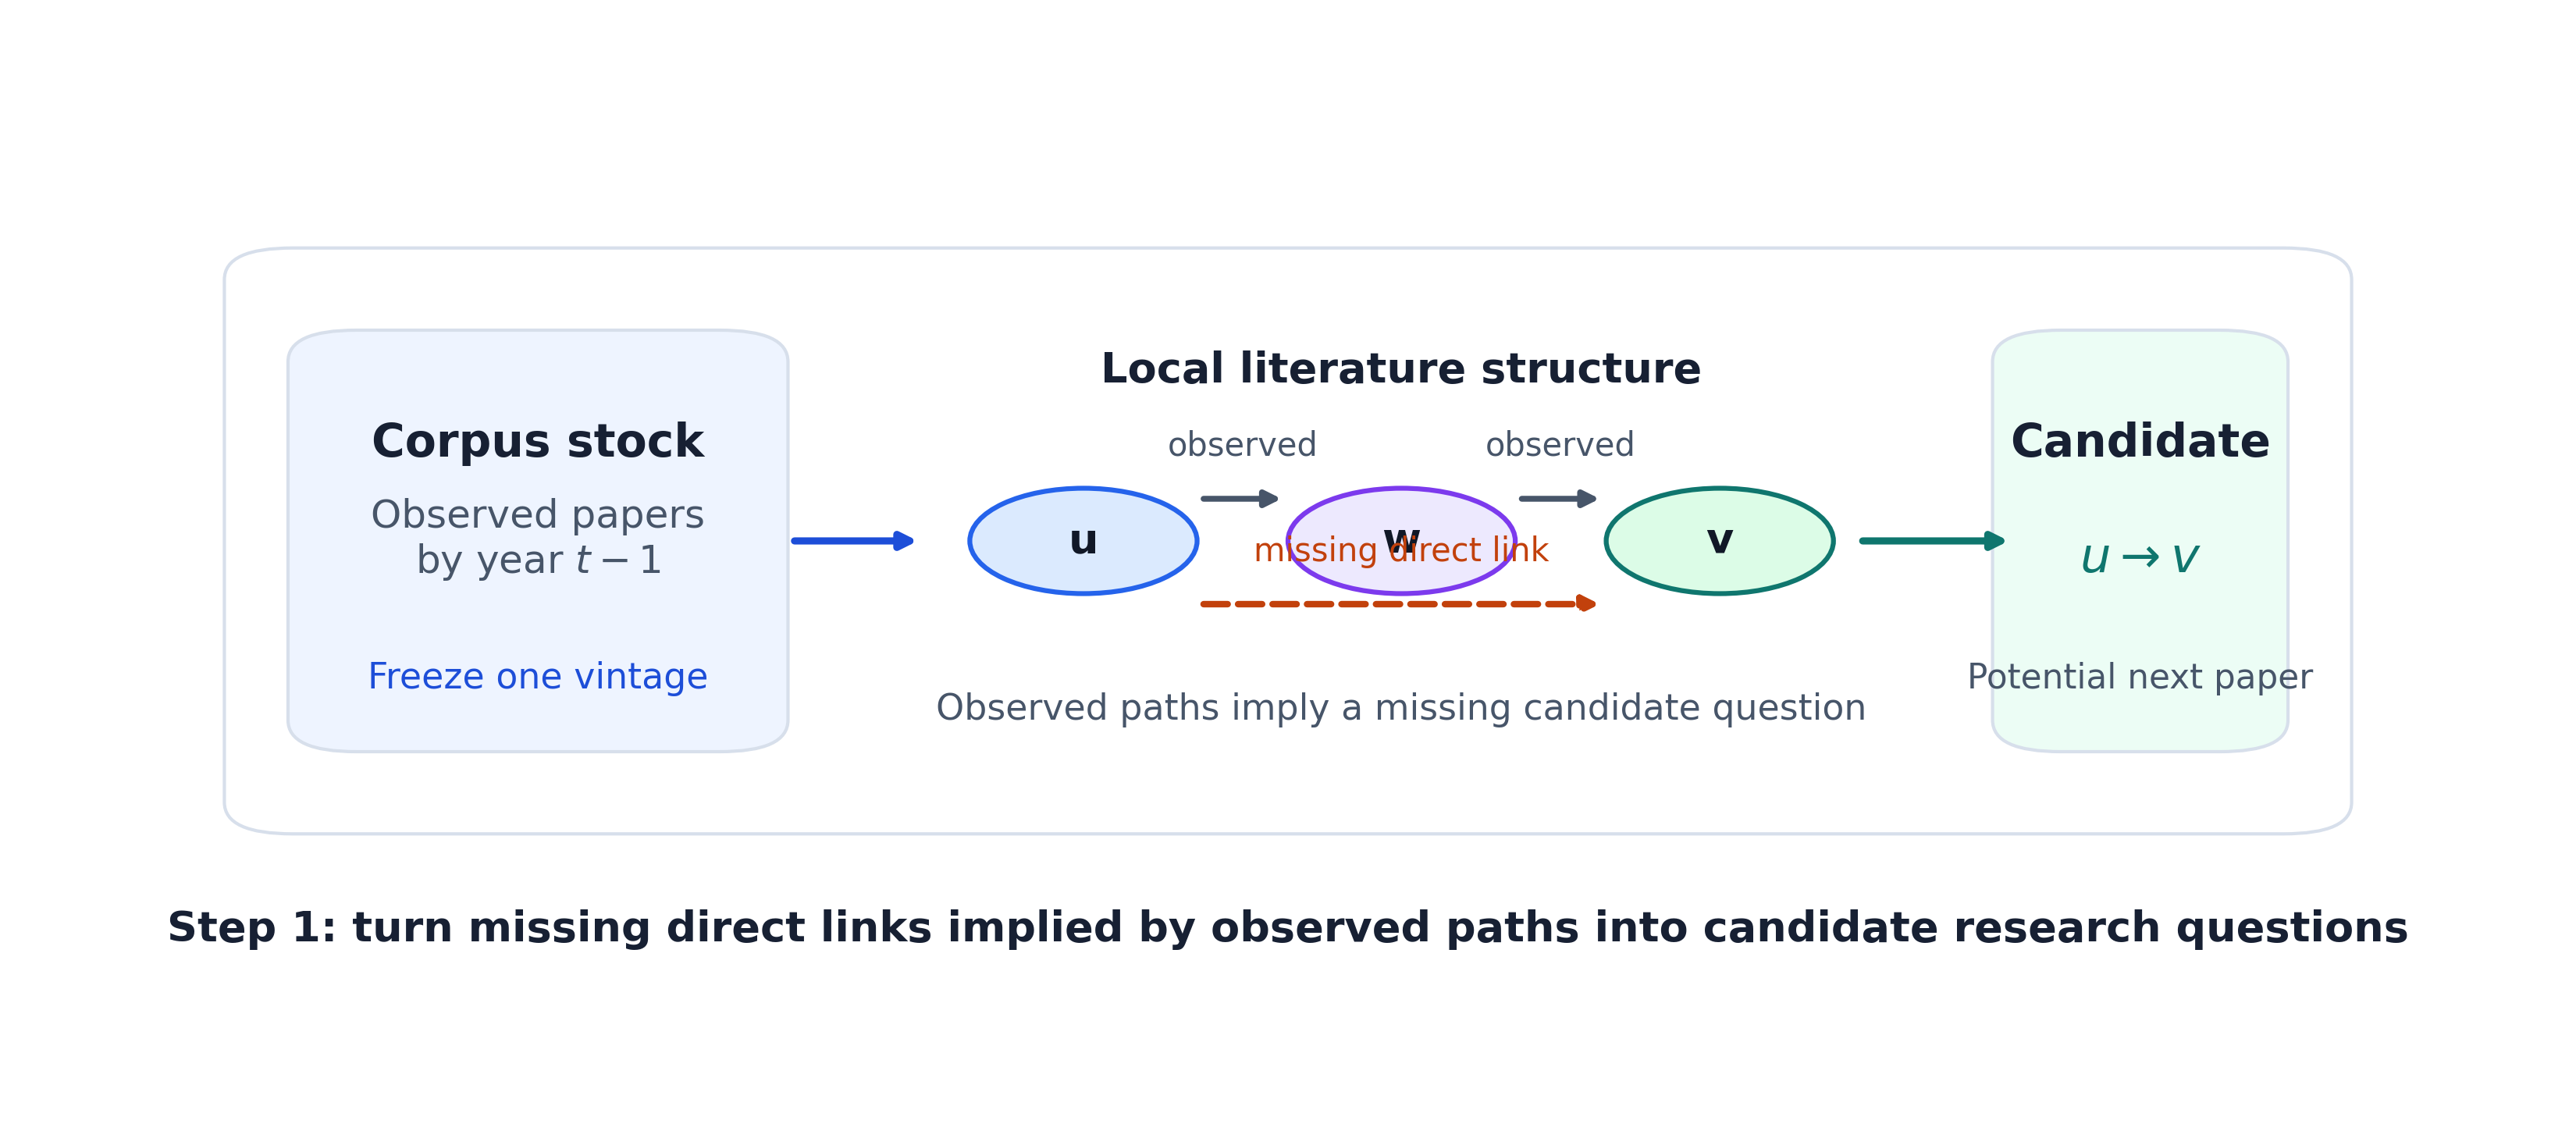
\includegraphics[width=0.90\linewidth]{method_build_step1_candidates.png}
\end{center}

\vspace{0.20em}
\begin{center}
\fcolorbox{DeckLine}{DeckSand}{\parbox{0.88\linewidth}{\centering
\small
\textcolor{DeckBlue}{\bfseries Freeze a vintage}
\hspace{0.5em}$\rightarrow$\hspace{0.5em}
\textcolor{DeckRose}{\bfseries Read the local gap}
\hspace{0.5em}$\rightarrow$\hspace{0.5em}
\textcolor{DeckTeal}{\bfseries Create a candidate next paper}
}}
\end{center}

\vspace{0.12em}
\begin{flushright}
\detailsbutton{app-candidate}
\end{flushright}
\end{frame}

\begin{frame}[label=main-score]{How the score works}
\begin{center}
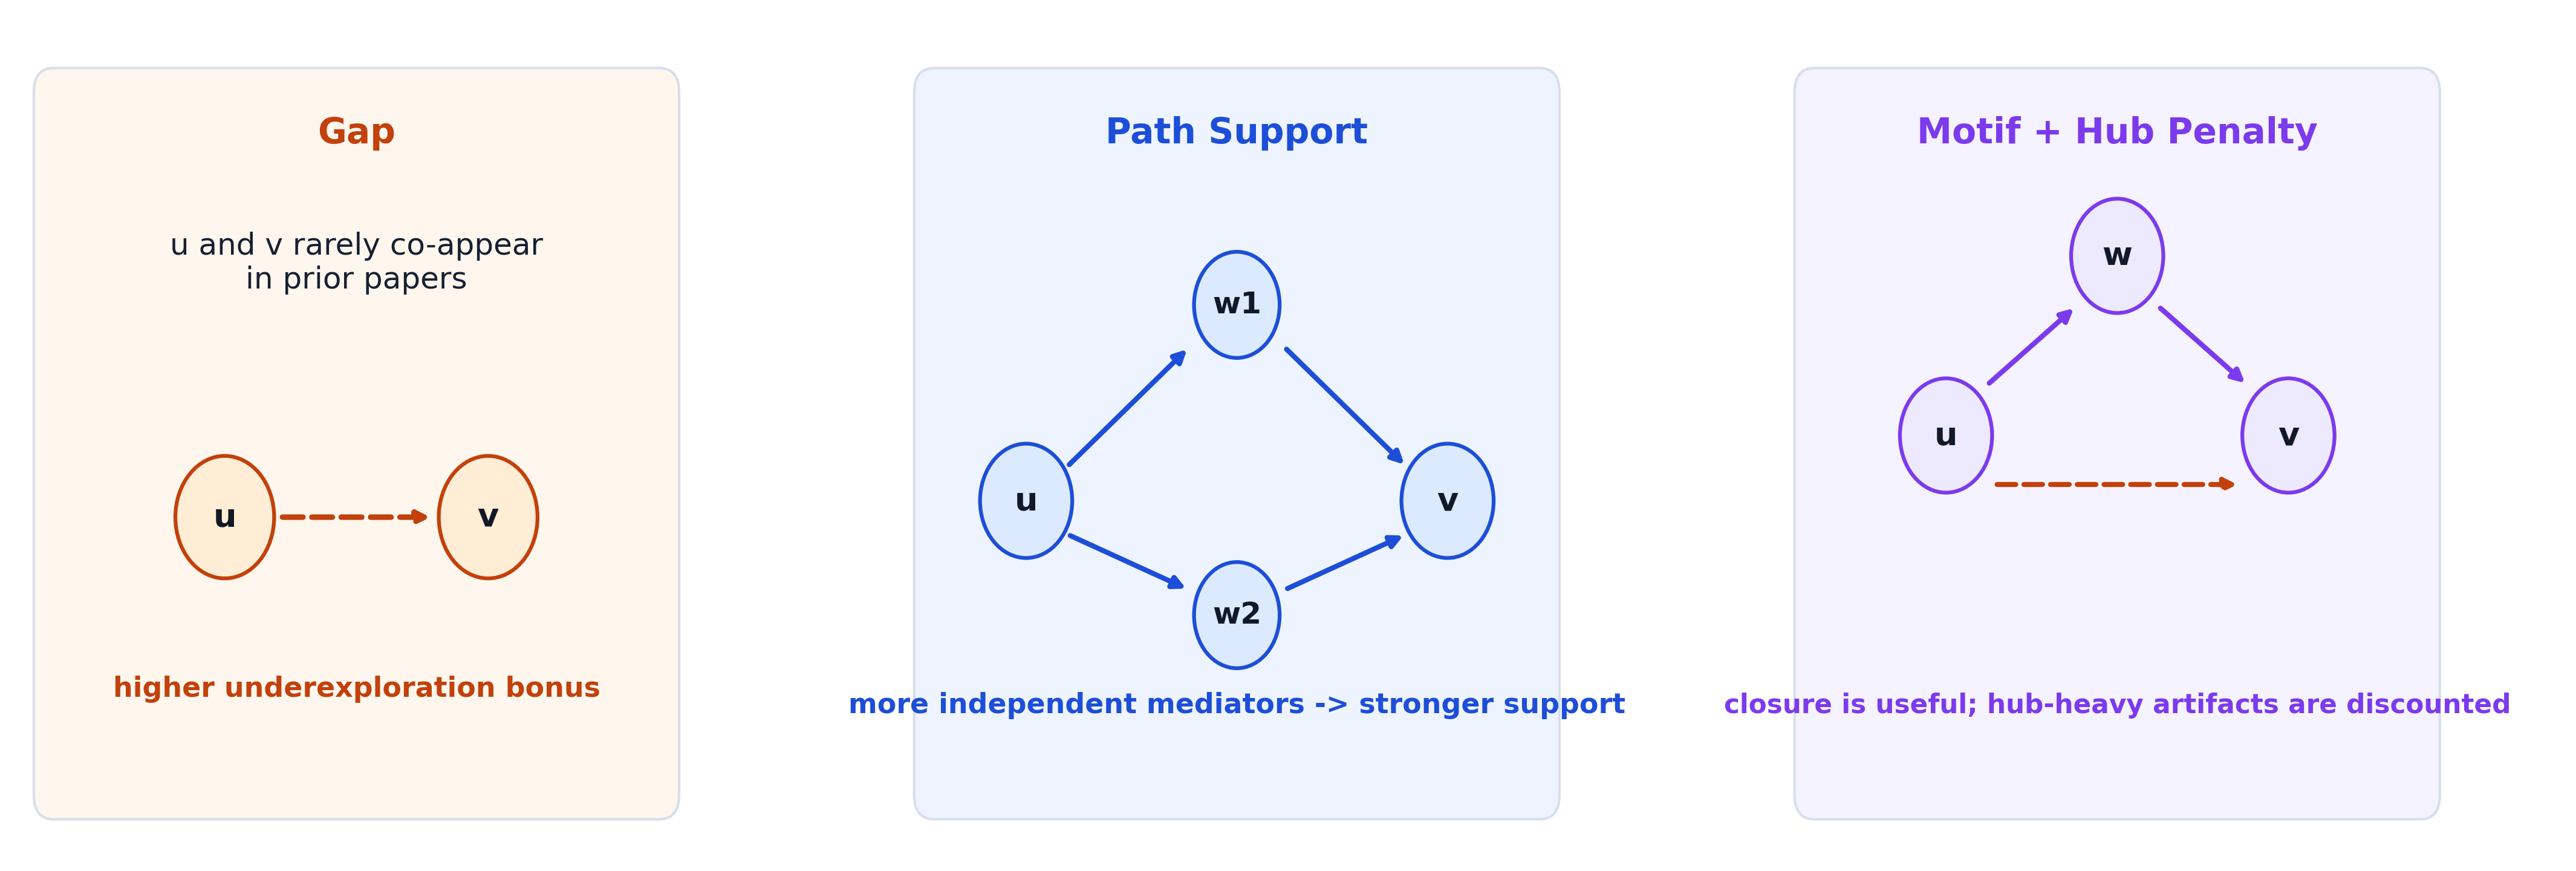
\includegraphics[width=0.90\linewidth]{method_build_step2_signals.png}
\end{center}

\vspace{0.18em}
\begin{center}
\fcolorbox{DeckLine}{DeckSand}{\parbox{0.90\linewidth}{\centering
\small
\textcolor{DeckWarn}{\bfseries Gap = openness}
\hspace{0.7em}\textbar\hspace{0.7em}
\textcolor{DeckBlue}{\bfseries Path support = plausibility}
\hspace{0.7em}\textbar\hspace{0.7em}
\textcolor{DeckRose}{\bfseries Hub discipline = not just popularity}
}}
\end{center}

\vspace{0.3em}
\begin{flushright}
\detailsbutton{app-score}
\end{flushright}
\end{frame}

\begin{frame}[label=main-test]{How we test it prospectively}
\begin{center}
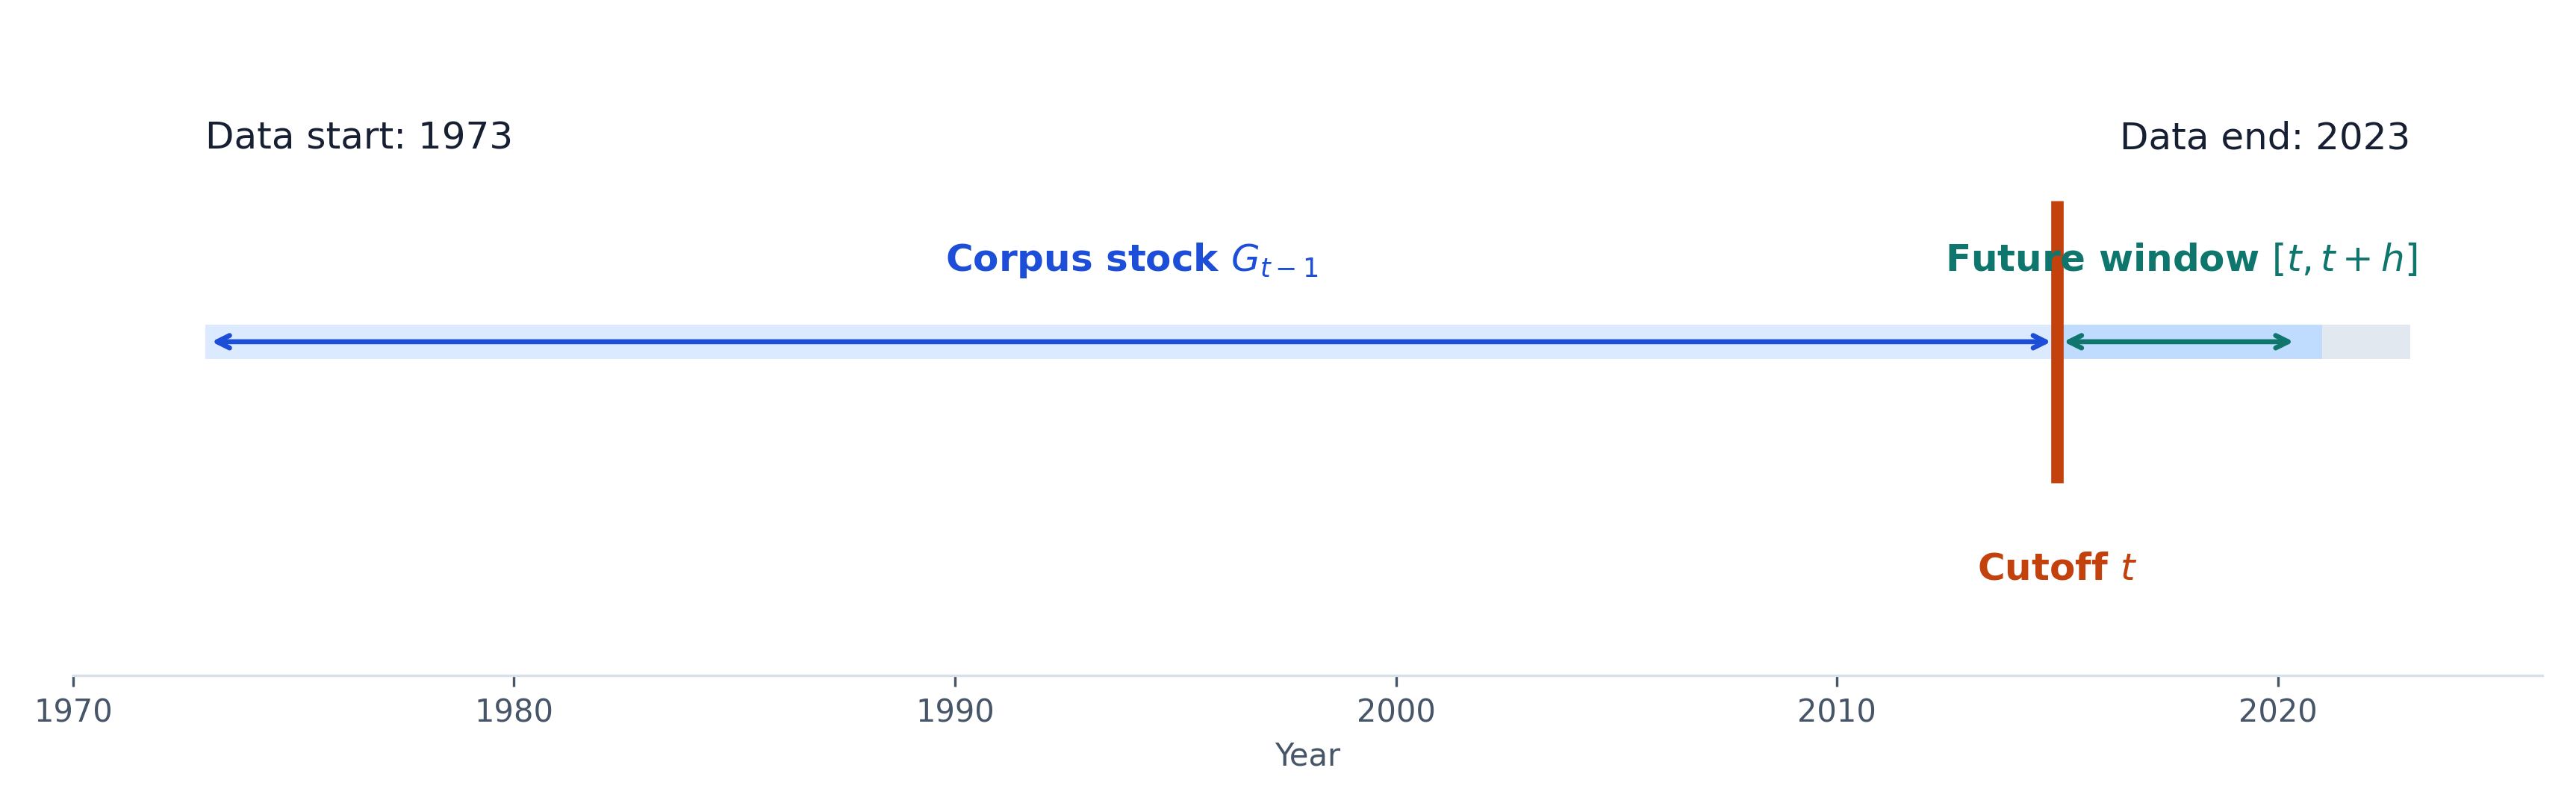
\includegraphics[width=0.90\linewidth]{corpus_stock_timeline.png}
\end{center}

\vspace{0.18em}
\begin{center}
\fcolorbox{DeckLine}{DeckSand}{\parbox{0.92\linewidth}{\centering
\small
\textcolor{DeckBlue}{\bfseries 1. Build \(G_{t-1}\)}
\hspace{0.55em}$\rightarrow$\hspace{0.55em}
\textcolor{DeckRose}{\bfseries 2. Rank links}
\hspace{0.55em}$\rightarrow$\hspace{0.55em}
\textcolor{DeckTeal}{\bfseries 3. Wait \(h\) years}
\hspace{0.55em}$\rightarrow$\hspace{0.55em}
\textcolor{DeckWarn}{\bfseries 4. Compare cleanly}
}}
\end{center}

\vspace{0.3em}
\begin{flushright}
\detailsbutton{app-eval}
\end{flushright}
\end{frame}

\begin{frame}[label=main-rolling]{Main result: honest benchmark}
\begin{columns}[T]
\column{0.60\linewidth}
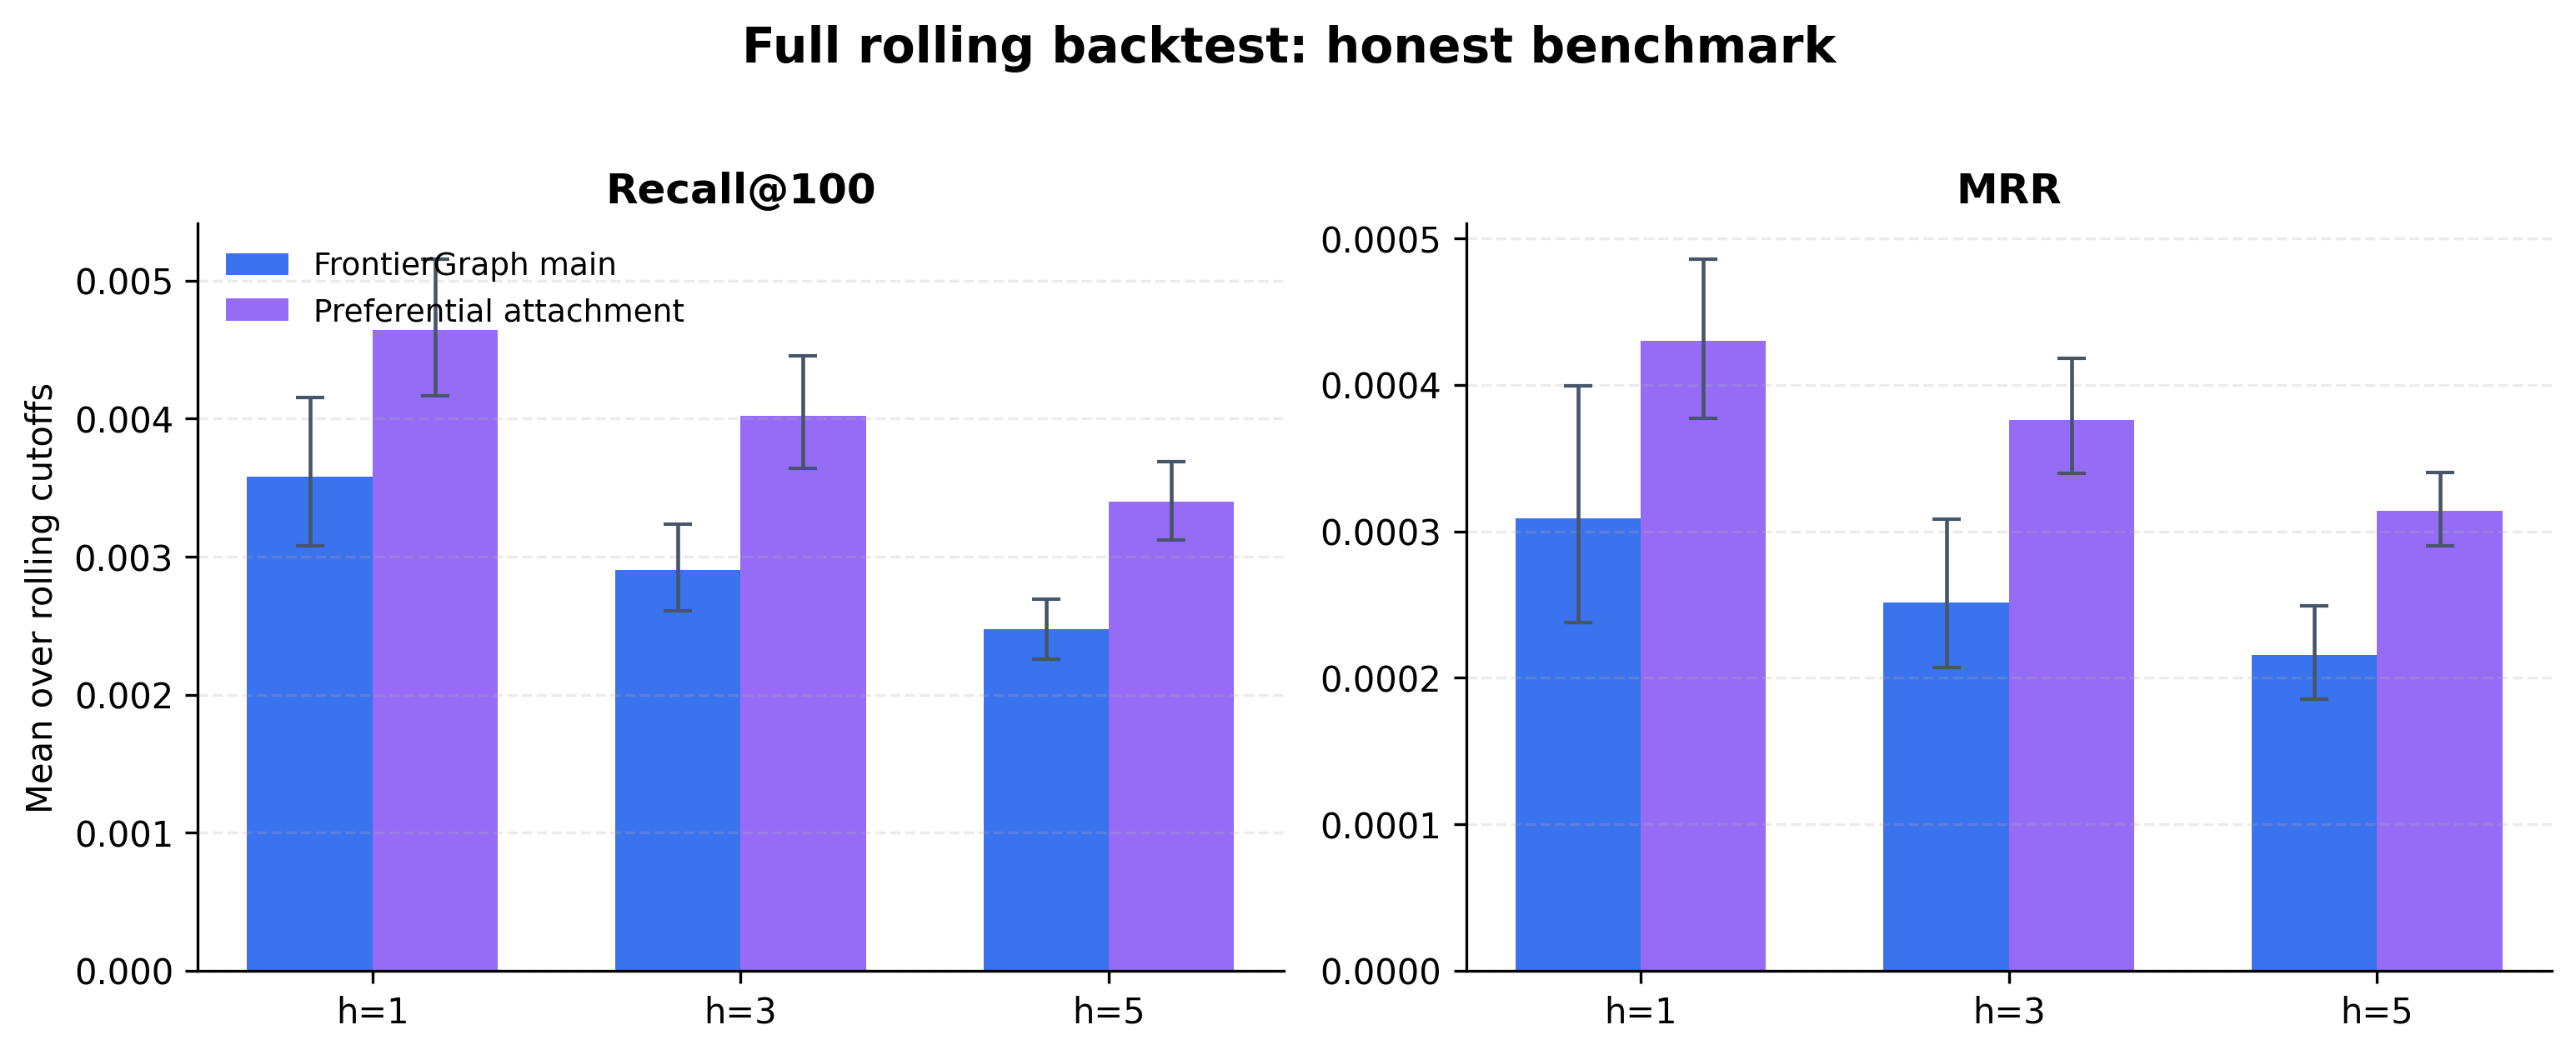
\includegraphics[width=\linewidth]{mainline_full_rolling_vs_pref.png}

\column{0.36\linewidth}
\small
\begin{itemize}
  \item[\color{DeckWarn}{\Large$\blacklozenge$}] Preferential attachment is stronger in the full rolling benchmark.
  \item[\color{DeckRose}{\Large$\blacklozenge$}] That mixed result is central, not a footnote.
  \item[\color{DeckBlue}{\Large$\blacklozenge$}] The paper's value depends on what transparent signals still add under more decision-relevant settings.
\end{itemize}

\vspace{0.4em}
\begin{flushright}
\detailsbutton{app-rolling}
\end{flushright}
\end{columns}
\end{frame}

\begin{frame}[label=main-whyinteresting]{Why the project is still scientifically interesting}
\begin{columns}[T]
\column{0.55\linewidth}
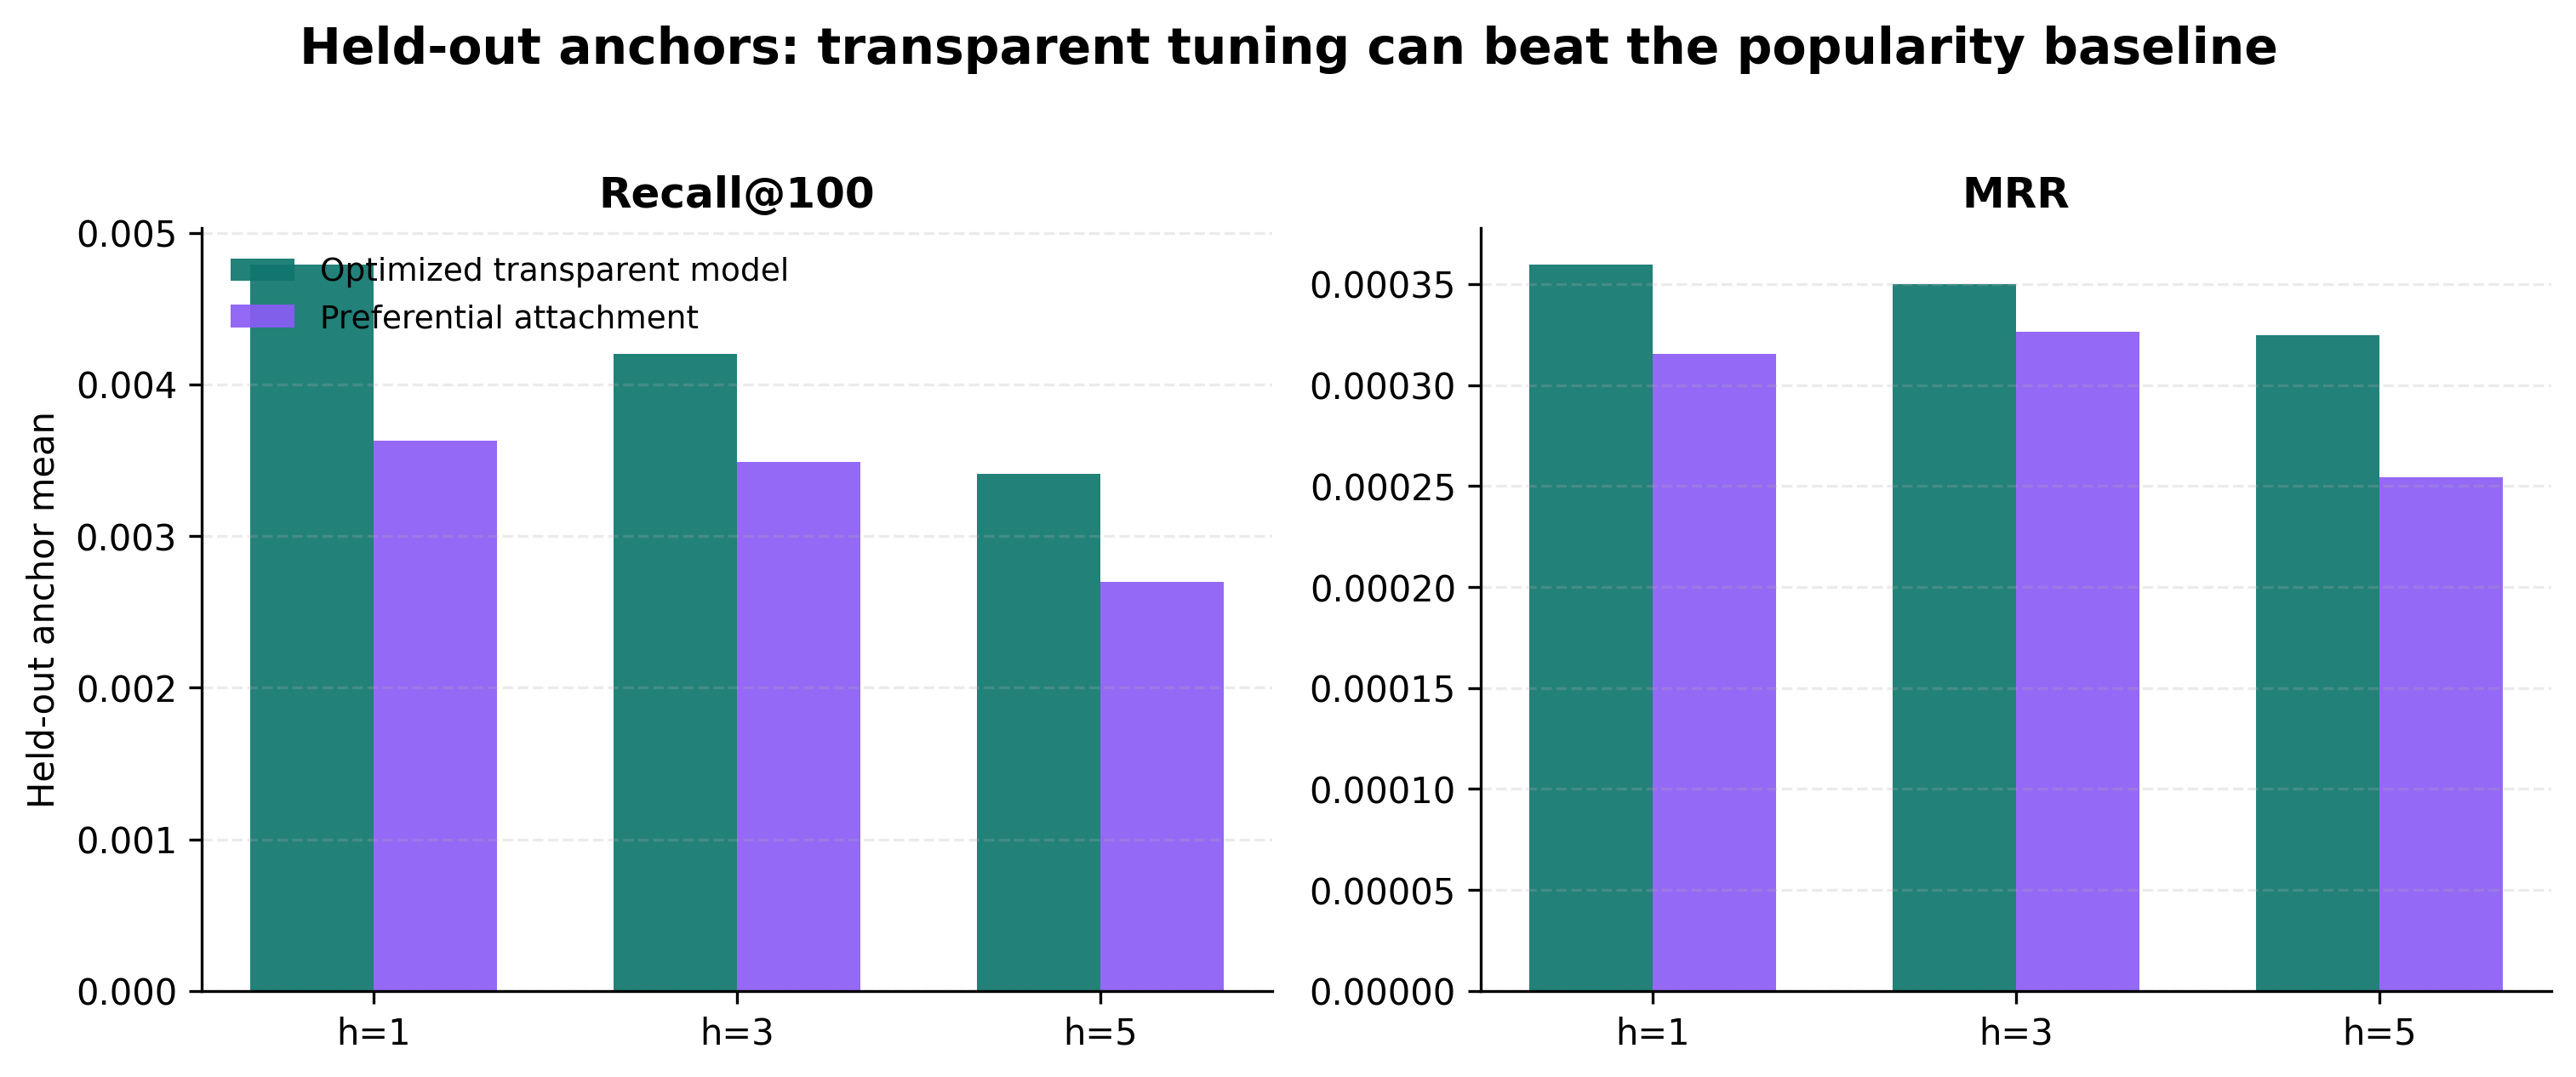
\includegraphics[width=\linewidth]{mainline_heldout_vs_pref.png}

\column{0.43\linewidth}
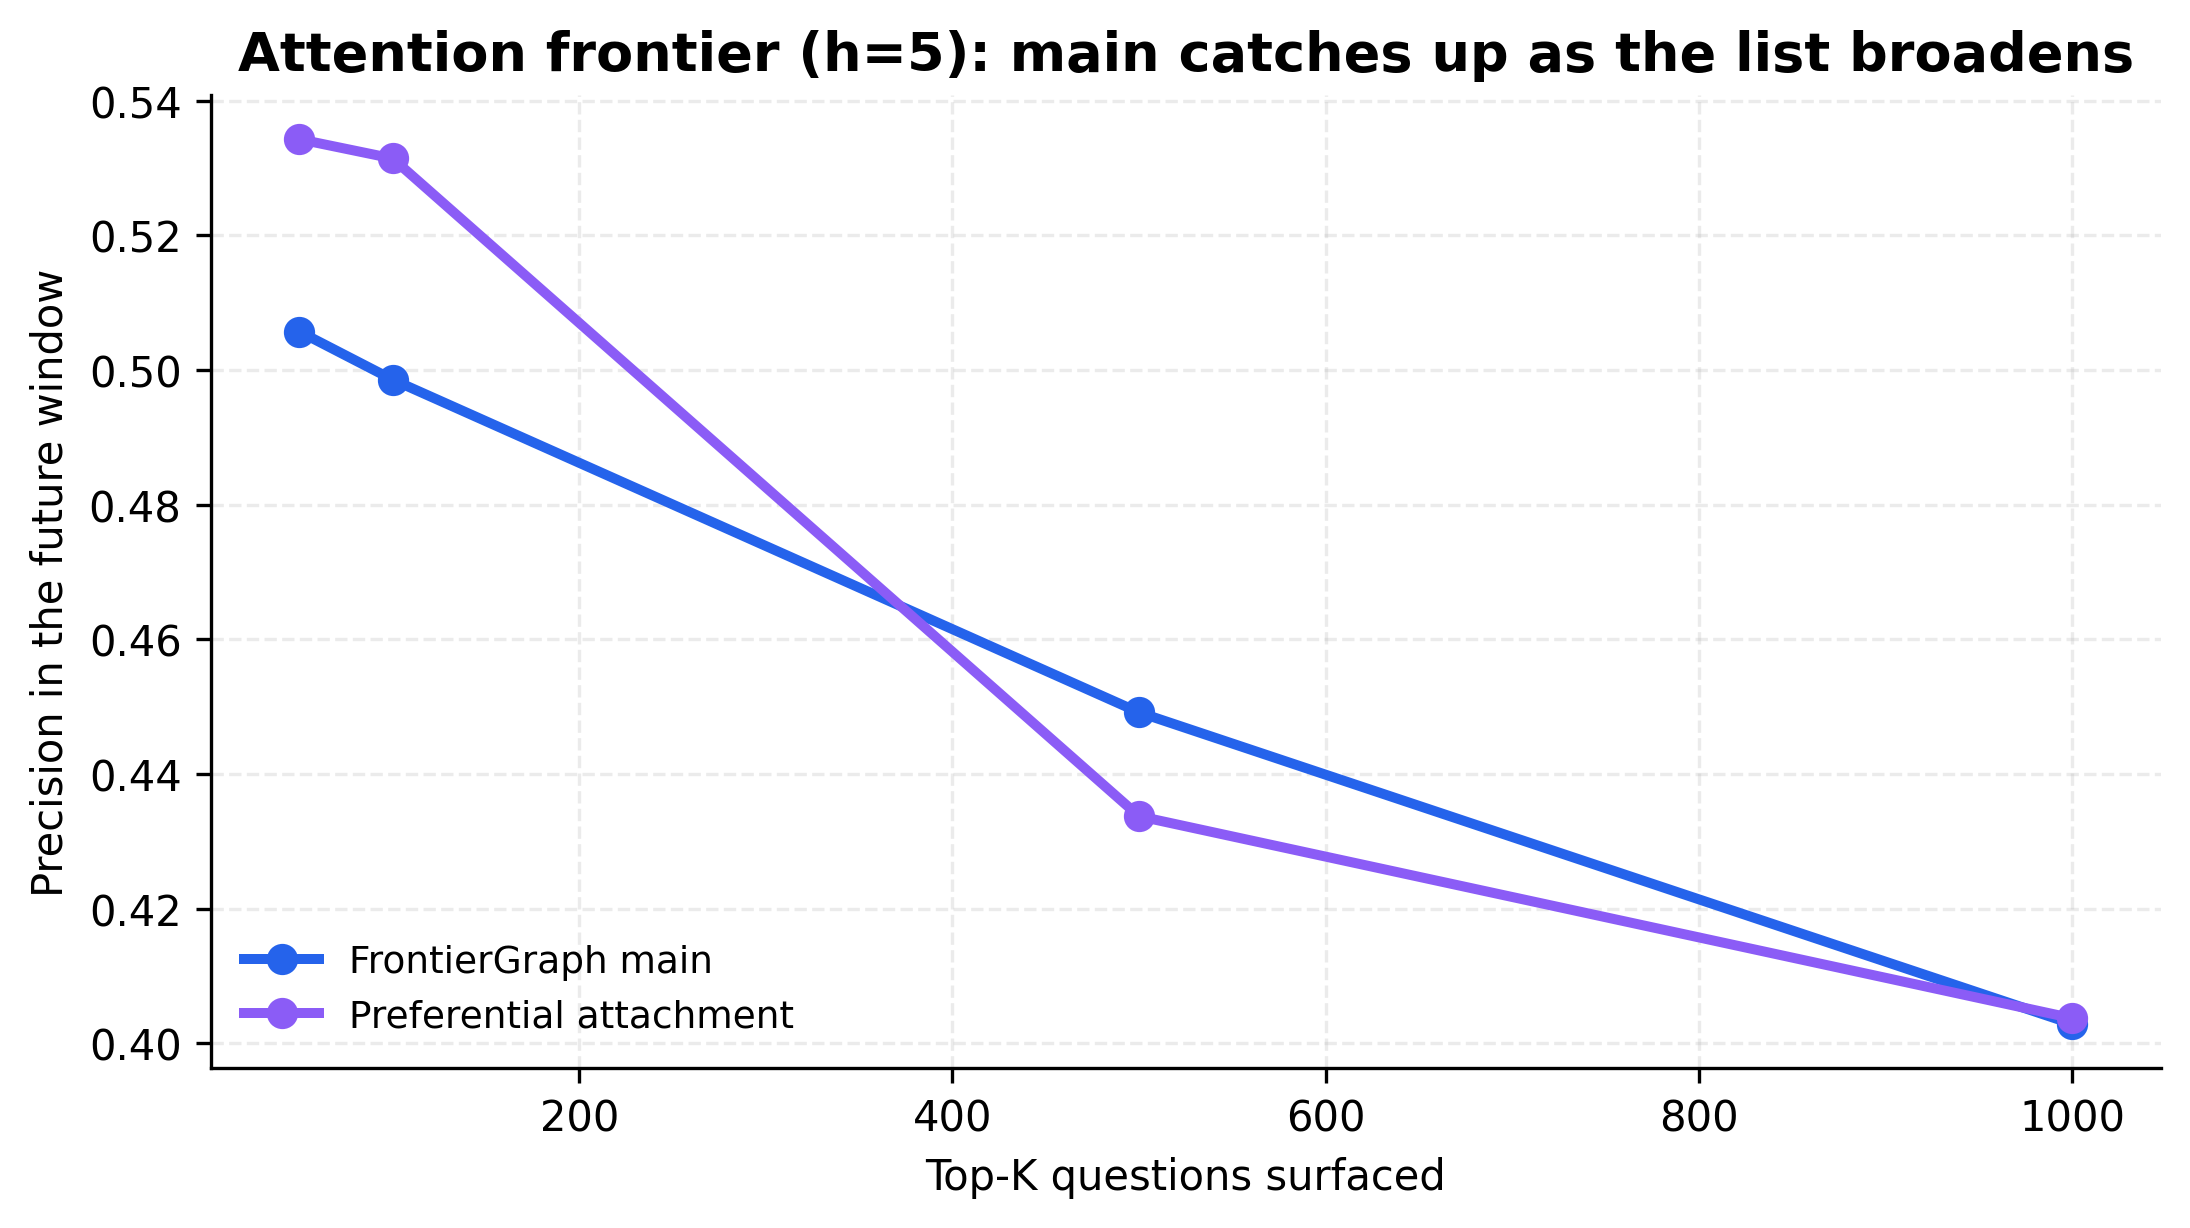
\includegraphics[width=\linewidth]{attention_allocation_frontier.png}
\end{columns}

\vspace{0.3em}
\small
\begin{itemize}
  \item[\color{DeckTeal}{\Large$\blacktriangleright$}] On held-out anchors, a tuned transparent model can beat the popularity baseline.
  \item[\color{DeckBlue}{\Large$\blacktriangleright$}] In broader top-\(K\) slices, the main model catches up and can slightly exceed preferential attachment.
  \item[\color{DeckRose}{\Large$\blacktriangleright$}] That makes the tool plausible as a screening layer even if popularity is hard to beat in the narrowest benchmark.
\end{itemize}

\detailsbutton{app-heldout}
\end{frame}

\begin{frame}[label=main-surfaces]{What kind of questions it surfaces}
\begin{columns}[T]
\column{0.54\linewidth}
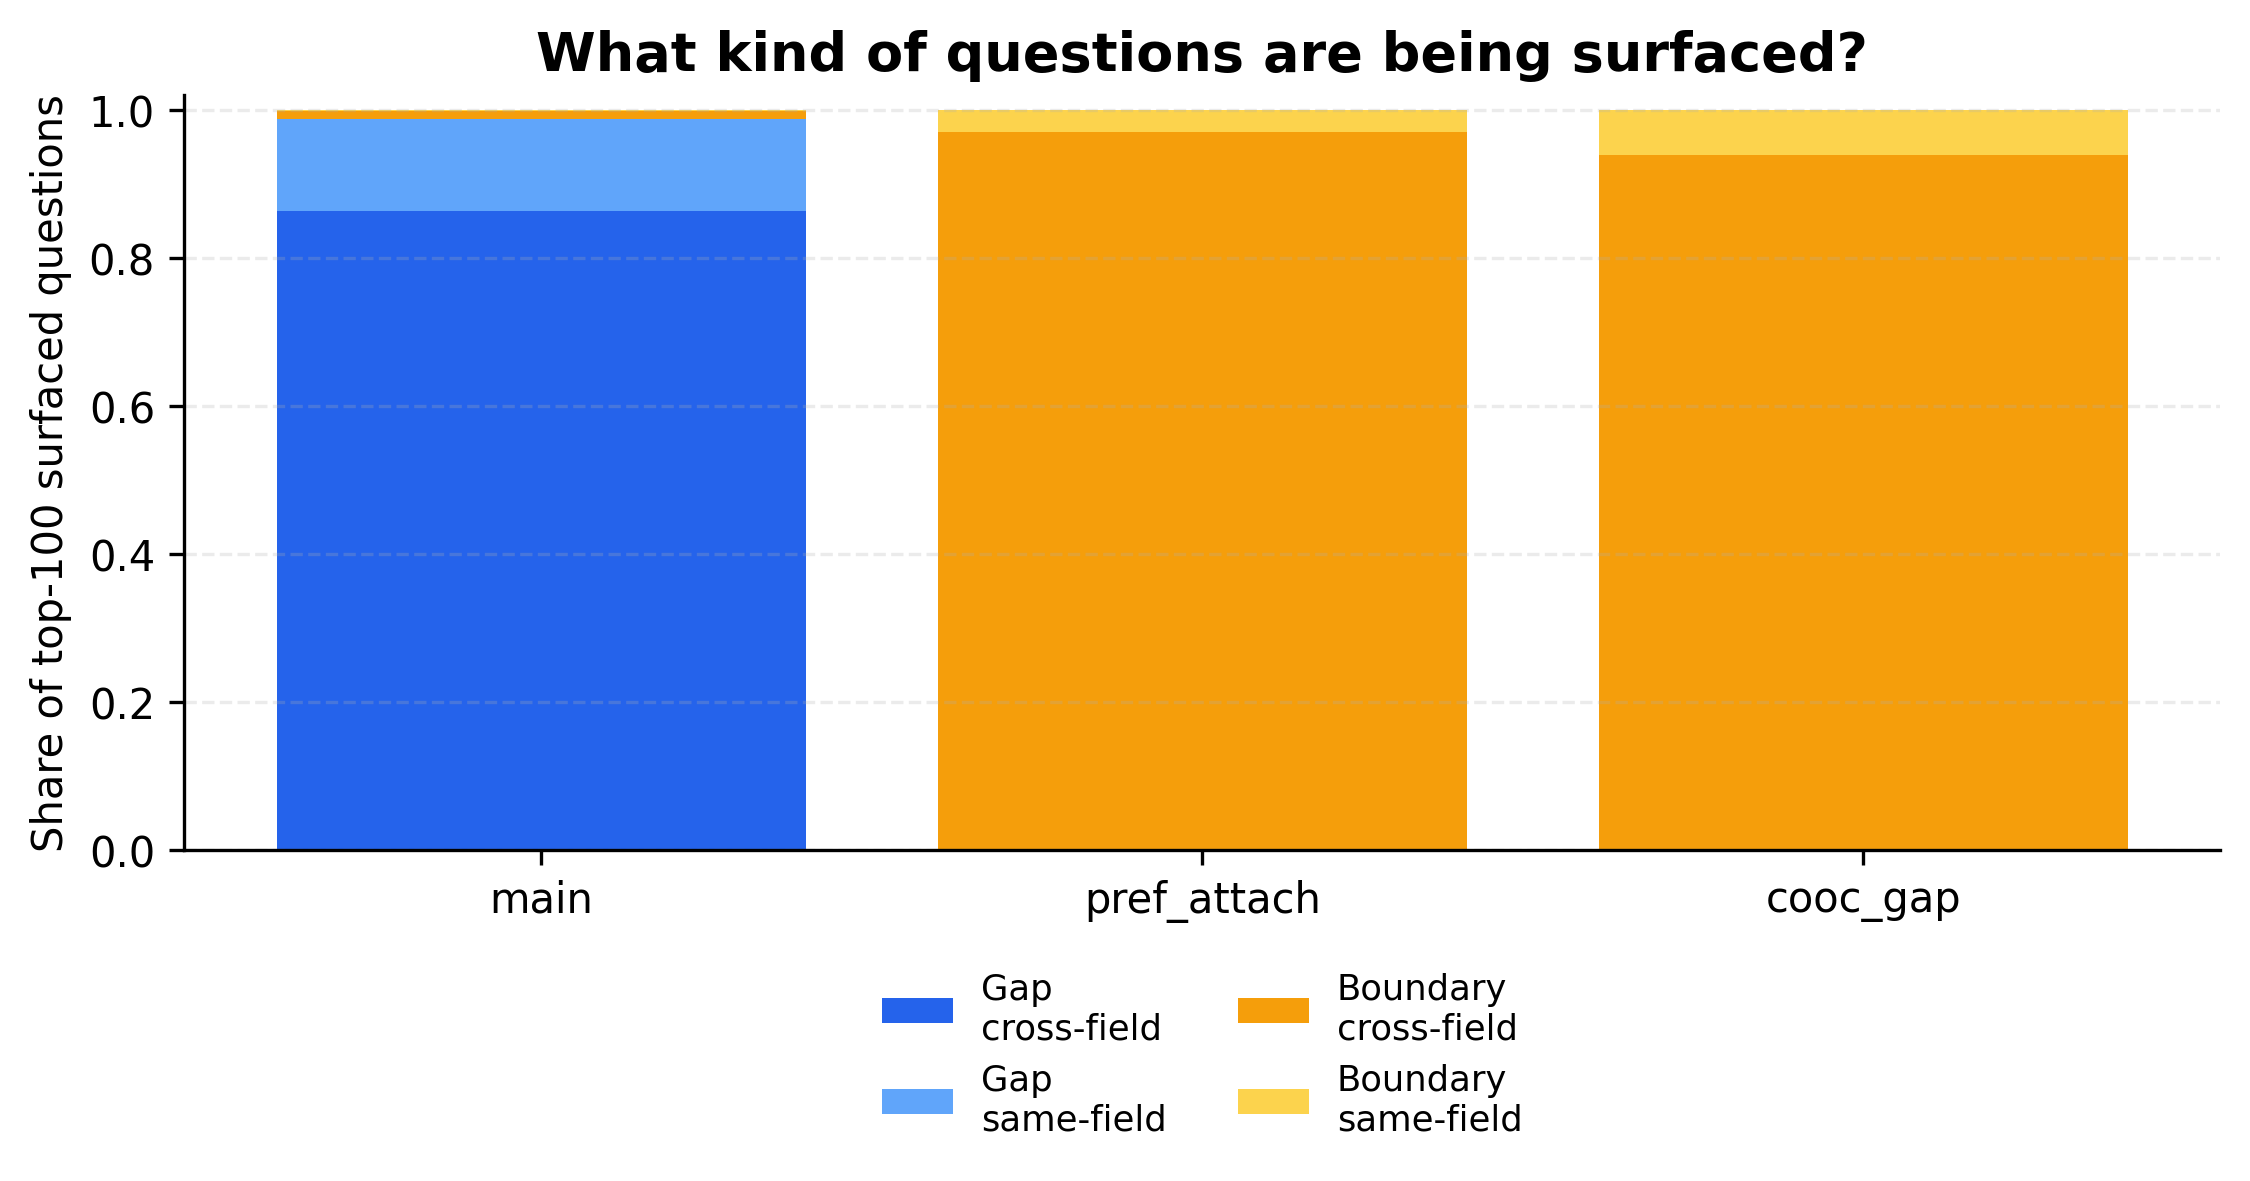
\includegraphics[width=\linewidth]{gap_boundary_mainline.png}

\column{0.42\linewidth}
\small
\begin{itemize}
  \item[\color{DeckBlue}{\Large$\star$}] The transparent model mostly surfaces \textbf{gap}-type questions rather than boundary-heavy popularity closures.
  \item[\color{DeckTeal}{\Large$\star$}] That is exactly the kind of object we want if the paper is about research allocation rather than pure forecast mimicry.
  \item[\color{DeckWarn}{\Large$\star$}] Boundary questions still matter, but they need separate evaluation because they are rarer and harder.
\end{itemize}

\vspace{0.7em}
\detailsbutton{app-gap}
\end{columns}
\end{frame}

\begin{frame}[label=main-examples]{Concrete examples from the current FrontierGraph layer}
\small
\begin{block}{Illustrative current outputs, not historical validation proof}
Examples of the kind of candidate next-paper questions the system surfaces today.
\end{block}

\vspace{0.35em}
\begin{columns}[T]
\column{0.32\linewidth}
\accentcard{DeckPeach}{3.00cm}{DeckWarn}{Public debt and CO\(_2\) emissions}{Debt stress can reshape investment and energy policy.\par\vspace{0.20em}\textbf{Start:} austerity or refinancing episodes.}

\column{0.32\linewidth}
\accentcard{DeckSoft}{3.00cm}{DeckBlue}{Monetary policy and energy consumption}{Monetary shocks move spending and production, but energy demand is rarely centered.\par\vspace{0.20em}\textbf{Start:} housing, durables, and sectoral energy use.}

\column{0.32\linewidth}
\accentcard{DeckMint}{3.00cm}{DeckTeal}{Urbanization and output growth}{Urbanization is often backgrounded rather than tested as the growth question itself.\par\vspace{0.20em}\textbf{Start:} regional urban expansion or city concentration.}
\end{columns}
\end{frame}

\begin{frame}[label=main-not]{What this tool is and is not}
\begin{columns}[T]
\column{0.48\linewidth}
\begin{block}{What it is}
\begin{itemize}
  \item A transparent screening aid
  \item A prospective research-allocation framework
  \item A way to inspect why a question was surfaced
\end{itemize}
\end{block}

\column{0.48\linewidth}
\begin{block}{What it is not}
\begin{itemize}
  \item Not causal truth
  \item Not a literature review
  \item Not a final verdict on what economics should study
\end{itemize}
\end{block}
\end{columns}

\vspace{0.45em}
\small
The scientific claim is predictive utility plus transparent decomposition, not algorithmic authority over the research agenda.
\end{frame}

\begin{frame}[label=main-artifact]{FrontierGraph as research artifact}
{\color{DeckMuted}\small The interface layer matters because it makes the research-allocation object inspectable, but it is downstream of the scientific core.}

\vspace{0.45em}
\begin{center}
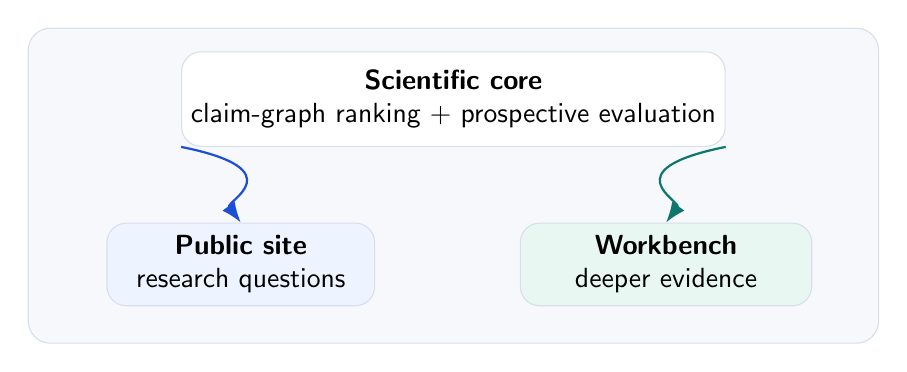
\begin{tikzpicture}[x=1cm,y=1cm]
  \node[
    draw=DeckLine,
    rounded corners=8pt,
    fill=DeckSand,
    minimum width=10.8cm,
    minimum height=4.0cm
  ] (panel) at (0,0) {};

  \node[
    draw=DeckLine,
    rounded corners=7pt,
    fill=white,
    minimum width=5.8cm,
    minimum height=1.20cm,
    align=center
  ] (core) at (0,1.10) {\textbf{Scientific core}\\claim-graph ranking + prospective evaluation};

  \node[
    draw=DeckLine,
    rounded corners=7pt,
    fill=DeckSoft,
    minimum width=3.4cm,
    minimum height=1.05cm,
    align=center
  ] (site) at (-2.7,-1.0) {\textbf{Public site}\\research questions};

  \node[
    draw=DeckLine,
    rounded corners=7pt,
    fill=DeckMint,
    minimum width=3.7cm,
    minimum height=1.05cm,
    align=center
  ] (app) at (2.7,-1.0) {\textbf{Workbench}\\deeper evidence};

  \draw[-{Latex[length=2.6mm]}, thick, color=DeckBlue] (core.south west) .. controls (-2.0,0.20) and (-2.9,-0.20) .. (site.north);
  \draw[-{Latex[length=2.6mm]}, thick, color=DeckTeal] (core.south east) .. controls (2.0,0.20) and (2.9,-0.20) .. (app.north);

\end{tikzpicture}
\end{center}

\vspace{0.30em}
\begin{center}
\fcolorbox{DeckLine}{DeckSand}{\parbox{0.92\linewidth}{\centering
\small
\textcolor{DeckBlue}{\bfseries Downstream artifacts}
\hspace{0.7em}\textbar\hspace{0.7em}
\textcolor{DeckTeal}{\bfseries Inspectable outputs}
\hspace{0.7em}\textbar\hspace{0.7em}
\textcolor{DeckWarn}{\bfseries Not the proof}
}}
\end{center}
\end{frame}

\begin{frame}[label=main-next]{Takeaways and next paper agenda}
\small
\begin{block}{Main takeaway}
FrontierGraph is best viewed as a transparent research-allocation tool: scientifically credible only if it is prospectively testable, interpretable, and honest about where popularity still wins.
\end{block}

\vspace{0.45em}
\begin{itemize}
  \item Update the evaluation on the larger public corpus.
  \item Run external transfer designs beyond the current internal benchmark.
  \item Add expert validation on surfaced questions.
  \item Freeze a prospective lockbox so the system can be judged out of sample in real time.
\end{itemize}
\end{frame}

\appendix

\begin{frame}[label=appendix-index]{Appendix index}
\small
\begin{columns}[T]
\column{0.49\linewidth}
\begin{itemize}
  \item \hyperlink{app-lit}{A1. Literature anchors}
  \item \hyperlink{app-foundation}{A2. Relation to the extraction foundation}
  \item \hyperlink{app-data}{A3. Data construction}
  \item \hyperlink{app-candidate}{A4. Candidate generation details}
  \item \hyperlink{app-score}{A5. Full score equation}
  \item \hyperlink{app-metrics}{A6. Metric definitions}
  \item \hyperlink{app-leakage}{A7. Leakage audit, CIs, significance}
  \item \hyperlink{app-rolling}{A8. Full rolling result table}
\end{itemize}

\column{0.49\linewidth}
\begin{itemize}
  \item \hyperlink{app-heldout}{A9. Held-out tuning / ablation}
  \item \hyperlink{app-attention}{A10. Attention-allocation frontier}
  \item \hyperlink{app-impact}{A11. Impact-weighted evaluation}
  \item \hyperlink{app-gap}{A12. Gap vs boundary decomposition}
  \item \hyperlink{app-heterogeneity}{A13. Field heterogeneity}
  \item \hyperlink{app-examples}{A14. More examples}
  \item \hyperlink{app-transfer}{A15. External transfer design}
  \item \hyperlink{app-lockbox}{A16. Expert validation + prospective lockbox}
\end{itemize}
\end{columns}
\end{frame}

\begin{frame}[label=app-lit]{A1. Literature anchors}
\appendixnav{main-why}
\vspace{0.4em}
\small
\textbf{Economics and metascience}
\begin{itemize}
  \item Bloom, Jones, Van Reenen, Webb (2020): ideas are getting harder to find.
  \item Jones (2009): burden of knowledge.
  \item Gentzkow, Kelly, Taddy (2019): text-as-data foundation.
\end{itemize}

\textbf{Science of science and network structure}
\begin{itemize}
  \item Swanson (1986): undiscovered public knowledge.
  \item Uzzi et al. (2013): atypical combinations and innovation.
  \item Liben-Nowell and Kleinberg (2007), Milo et al. (2002): link prediction and motifs.
\end{itemize}
\end{frame}

\begin{frame}[label=app-foundation]{A2. Relation to the Causal Claims extraction foundation}
\appendixnav{main-what}
\vspace{0.4em}
\small
\begin{itemize}
  \item The extraction backbone builds on \emph{Causal Claims in Economics} and the related \texttt{causal.claims} project.
  \item That foundational layer extracts paper-local graph structure from economics papers.
  \item FrontierGraph is a downstream layer that adds:
  \begin{itemize}
    \item candidate-question ranking,
    \item prospective evaluation,
    \item a public research-allocation interface.
  \end{itemize}
  \item The paper should be clear that the current product and the original extraction paper are related, but not the same object.
\end{itemize}
\end{frame}

\begin{frame}[label=app-data]{A3. Data construction: evaluated corpus vs current public build}
\appendixnav{main-test}
\vspace{0.35em}
\begin{columns}[T]
\column{0.48\linewidth}
\begin{block}{Evaluated vintage-backtest corpus}
\small
\begin{itemize}
  \item 30,896 papers
  \item 856 concept codes
  \item 420,000 directed edges
  \item 1973--2023
\end{itemize}
\end{block}

\column{0.48\linewidth}
\begin{block}{Current public FrontierGraph layer}
\small
\begin{itemize}
  \item 242,595 published papers
  \item 1,762,898 extracted concept instances
  \item 1,443,407 extracted edges
  \item 99,627 candidate questions screened
\end{itemize}
\end{block}
\end{columns}

\vspace{0.4em}
\small
Hybrid deck logic: the research-allocation framing comes from the current FrontierGraph layer, while the strongest existing prospective evidence still comes from the smaller validated stack.
\end{frame}

\begin{frame}[label=app-candidate]{A4. Candidate generation details}
\appendixnav{main-candidates}
\vspace{0.35em}
\begin{columns}[T]
\column{0.56\linewidth}
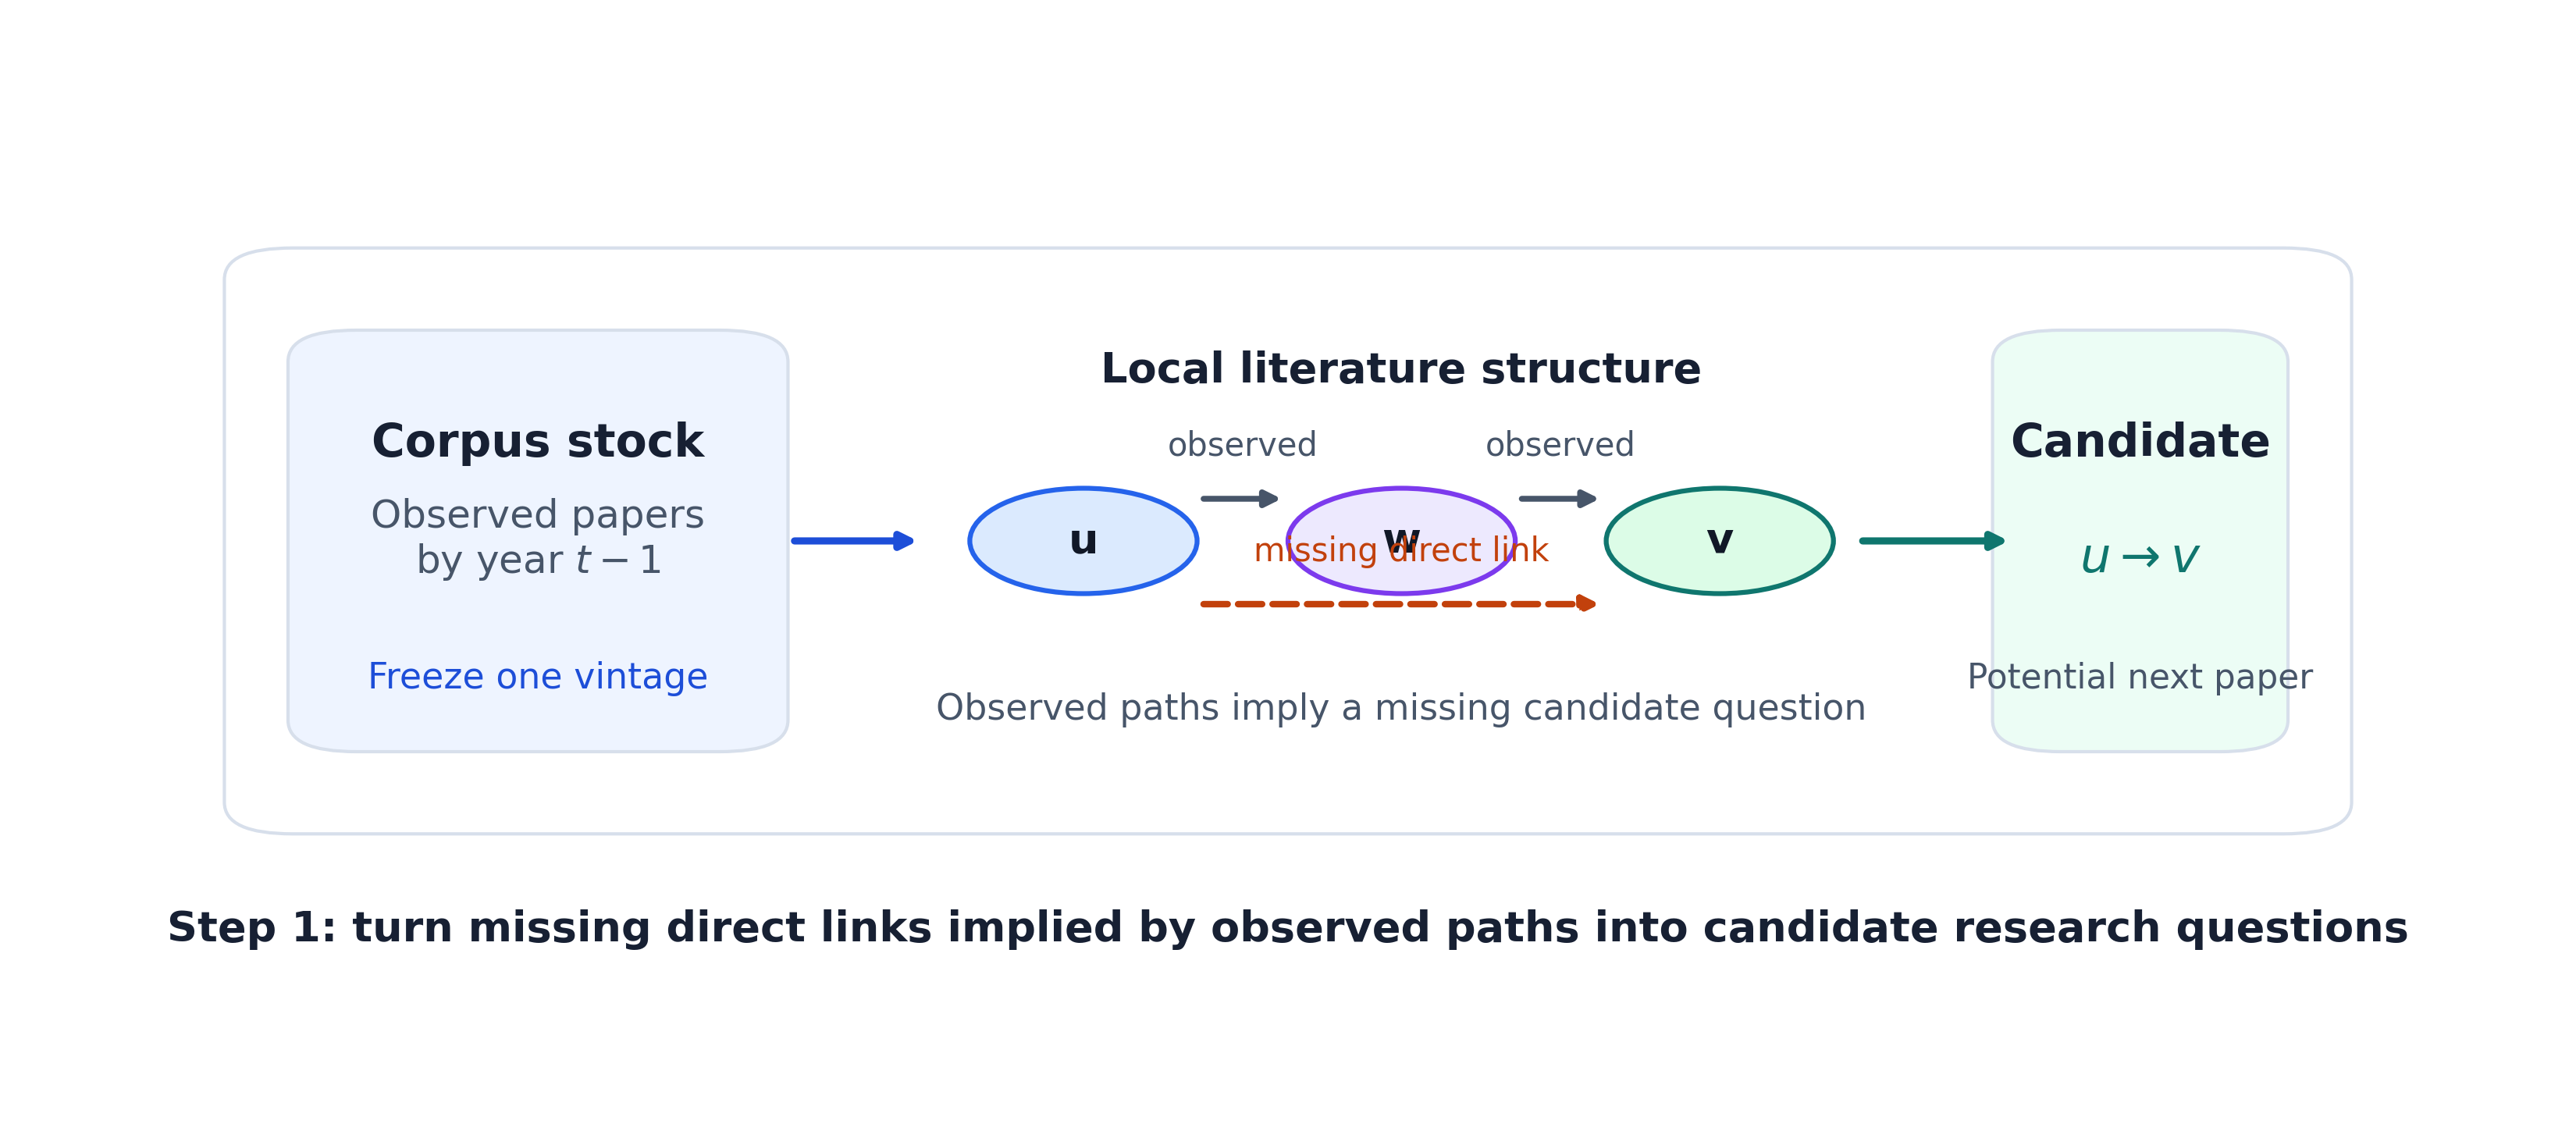
\includegraphics[width=\linewidth]{method_build_step1_candidates.png}

\column{0.40\linewidth}
\small
\begin{itemize}
  \item Freeze observed edges at \(t-1\).
  \item Enumerate absent \(u \rightarrow v\) links implied by local paths.
  \item Keep mediator provenance for every candidate.
  \item This is a candidate-generation step, not yet the final score.
\end{itemize}
\end{columns}
\end{frame}

\begin{frame}[label=app-score]{A5. Full score equation and component definitions}
\appendixnav{main-score}
\vspace{0.3em}
\begin{columns}[T]
\column{0.58\linewidth}
\small
\resizebox{\linewidth}{!}{$
\text{Score}(u\rightarrow v)=
\alpha\,\text{PathSupport}
\;+\;
\beta\,\text{GapBonus}
\;+\;
\gamma\,\text{MotifBonus}
\;-\;
\delta\,\text{HubPenalty}
$}

\vspace{0.2em}
\begin{itemize}
  \item \textbf{Path support}: evidence from \(u \rightarrow w \rightarrow v\) patterns and mediator structure.
  \item \textbf{Gap bonus}: reward absent or rare direct co-occurrence.
  \item \textbf{Motif bonus}: reward plausible structural closure.
  \item \textbf{Hub penalty}: avoid collapse into pure popularity effects.
\end{itemize}

\column{0.36\linewidth}
\includegraphics[width=\linewidth]{score_decomposition_example.png}
\end{columns}
\end{frame}

\begin{frame}[label=app-metrics]{A6. Metric definitions and why the numbers are small}
\appendixnav{main-test}
\vspace{0.35em}
\small
\begin{itemize}
  \item \textbf{Recall@100}: among all future realized links at a cutoff, what share appear in the top 100 ranked candidates?
  \item \textbf{MRR}: average reciprocal rank of the first realized true link.
  \item These values are small because the candidate space is enormous; the relevant comparison is against random and against strong baselines.
\end{itemize}

\vspace{0.5em}
\begin{tabular}{lccc}
\toprule
Setting & Random benchmark & Main & Pref.\ attach. \\
\midrule
Recall@100 (h=1) & $\approx 0$ & 0.00358 & 0.00465 \\
MRR (h=1) & $\approx 0$ & 0.000309 & 0.000430 \\
\bottomrule
\end{tabular}
\end{frame}

\begin{frame}[label=app-leakage]{A7. Leakage audit, confidence intervals, significance}
\appendixnav{main-test}
\vspace{0.35em}
\begin{columns}[T]
\column{0.56\linewidth}
\includegraphics[width=\linewidth]{../outputs/paper/02_eval/ci_recall_at_100.png}

\column{0.40\linewidth}
\small
\begin{itemize}
  \item Training data is frozen at each cutoff.
  \item Positive links in the evaluation window are excluded from the training graph.
  \item Report bootstrap confidence intervals over cutoffs.
  \item Use paired tests against preferential attachment rather than single-point claims.
\end{itemize}
\end{columns}
\end{frame}

\begin{frame}[label=app-rolling]{A8. Full rolling result table}
\appendixnav{main-rolling}
\vspace{0.45em}
\small
\begin{tabular}{lcccc}
\toprule
Horizon & Main R@100 & Pref.\ R@100 & Main MRR & Pref.\ MRR \\
\midrule
$h=1$ & 0.00358 & 0.00465 & 0.000309 & 0.000430 \\
$h=3$ & 0.00291 & 0.00402 & 0.000251 & 0.000376 \\
$h=5$ & 0.00248 & 0.00340 & 0.000215 & 0.000314 \\
\bottomrule
\end{tabular}

\vspace{0.6em}
\small
\begin{itemize}
  \item Honest reading: the full rolling benchmark still favors popularity.
  \item The scientific value of the paper depends on being explicit about that.
\end{itemize}
\end{frame}

\begin{frame}[label=app-heldout]{A9. Held-out tuning and ablation path}
\appendixnav{main-whyinteresting}
\vspace{0.35em}
\begin{columns}[T]
\column{0.58\linewidth}
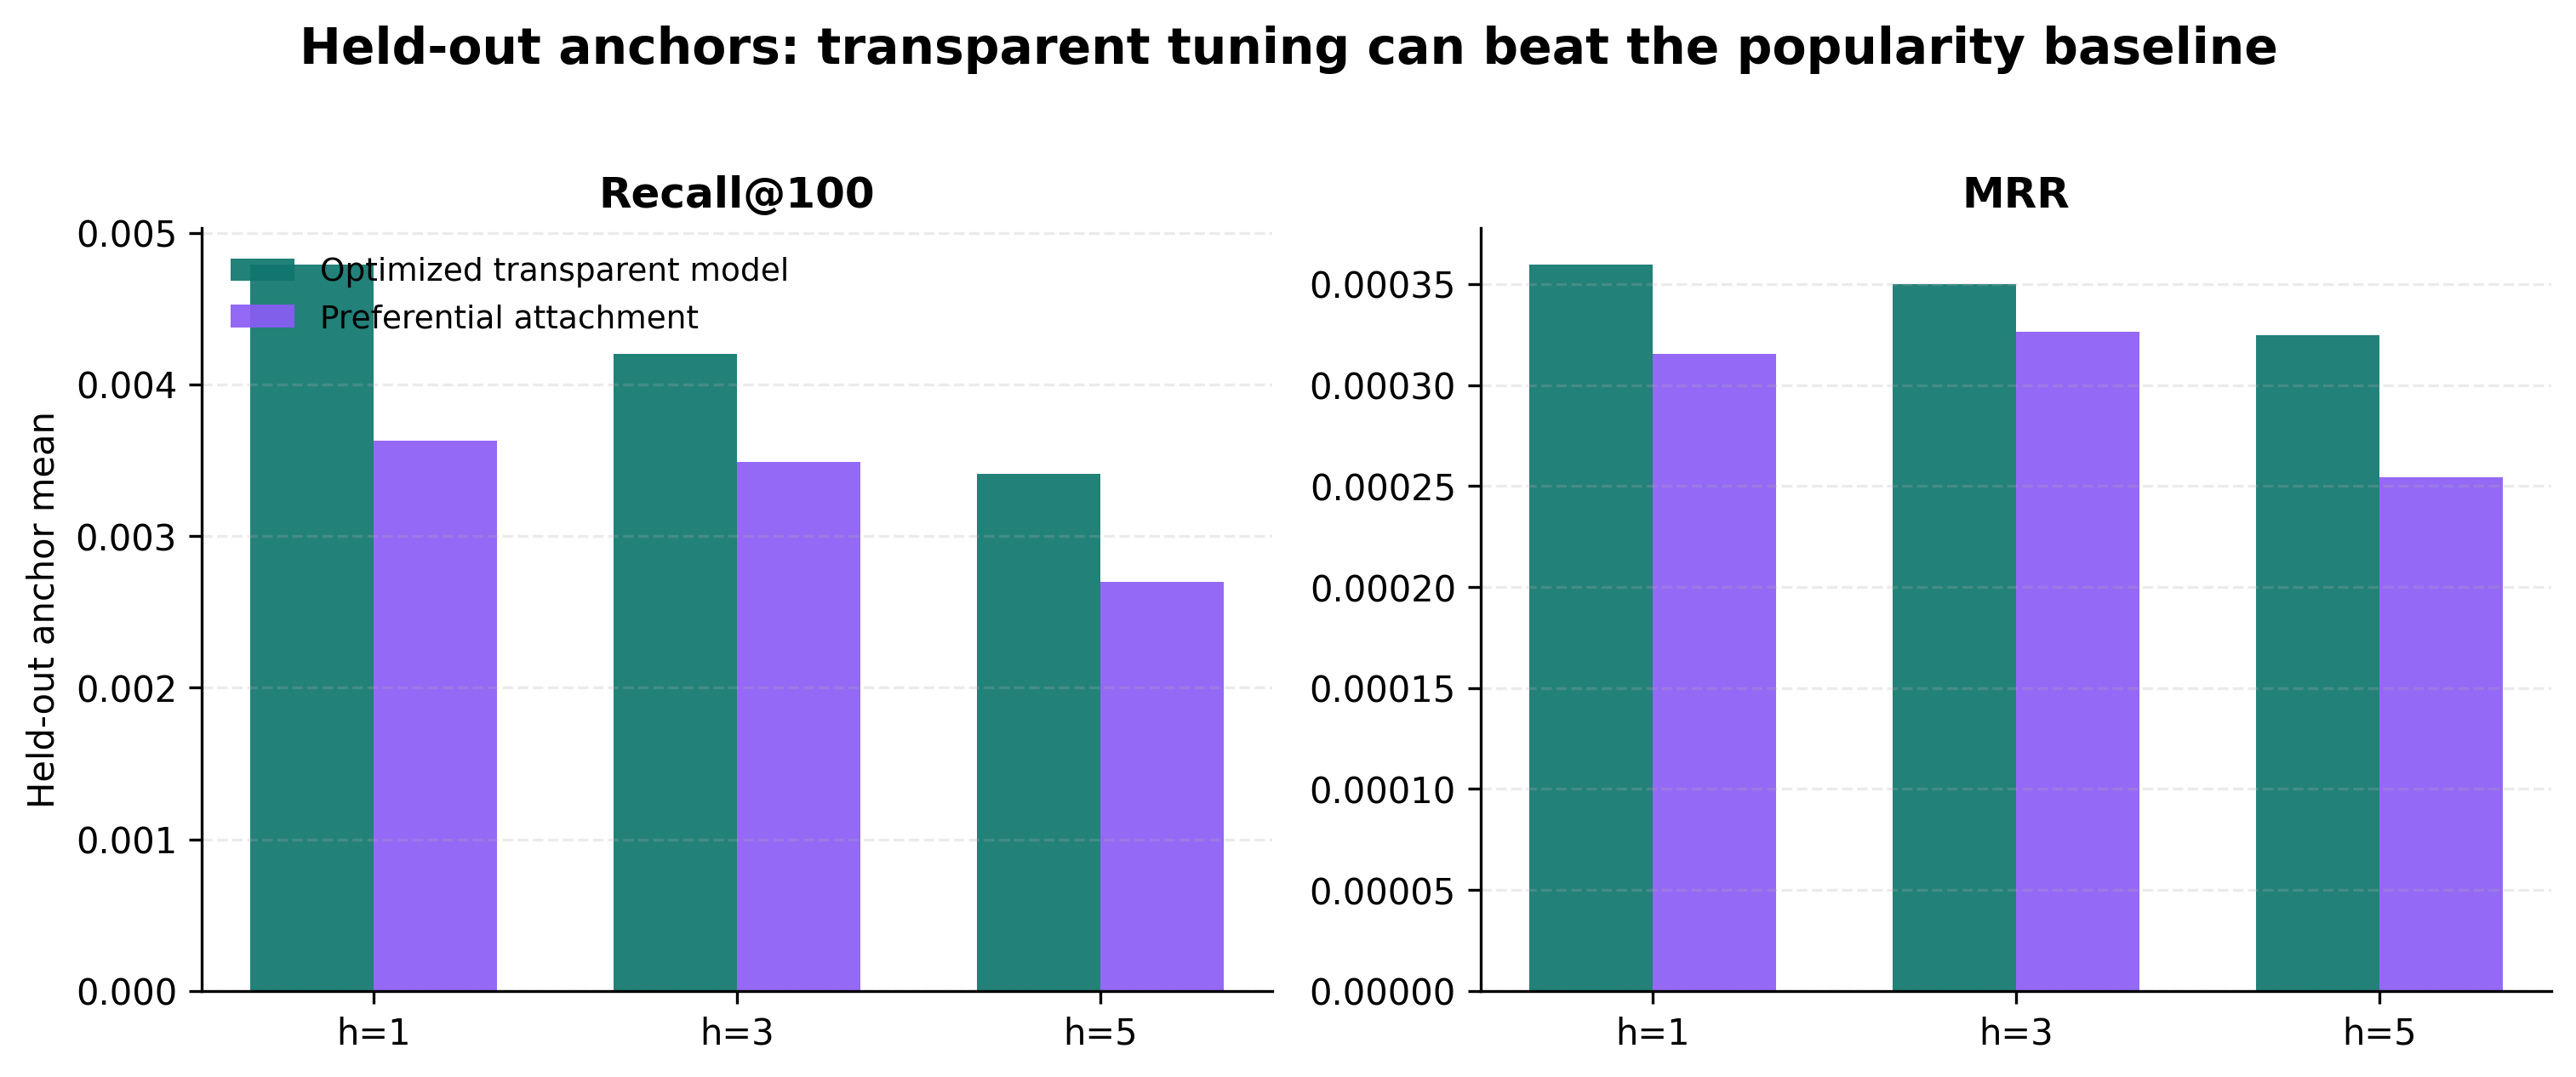
\includegraphics[width=\linewidth]{mainline_heldout_vs_pref.png}

\column{0.38\linewidth}
\small
\begin{itemize}
  \item Held-out anchor years are much smaller, but closer to a decision-use setting.
  \item Temporal weighting, stability, and field-aware hub control matter.
  \item This is not proof of general dominance, but it does show the transparent model can close the gap.
\end{itemize}
\end{columns}
\end{frame}

\begin{frame}[label=app-attention]{A10. Attention-allocation frontier}
\appendixnav{main-whyinteresting}
\vspace{0.35em}
\begin{columns}[T]
\column{0.58\linewidth}
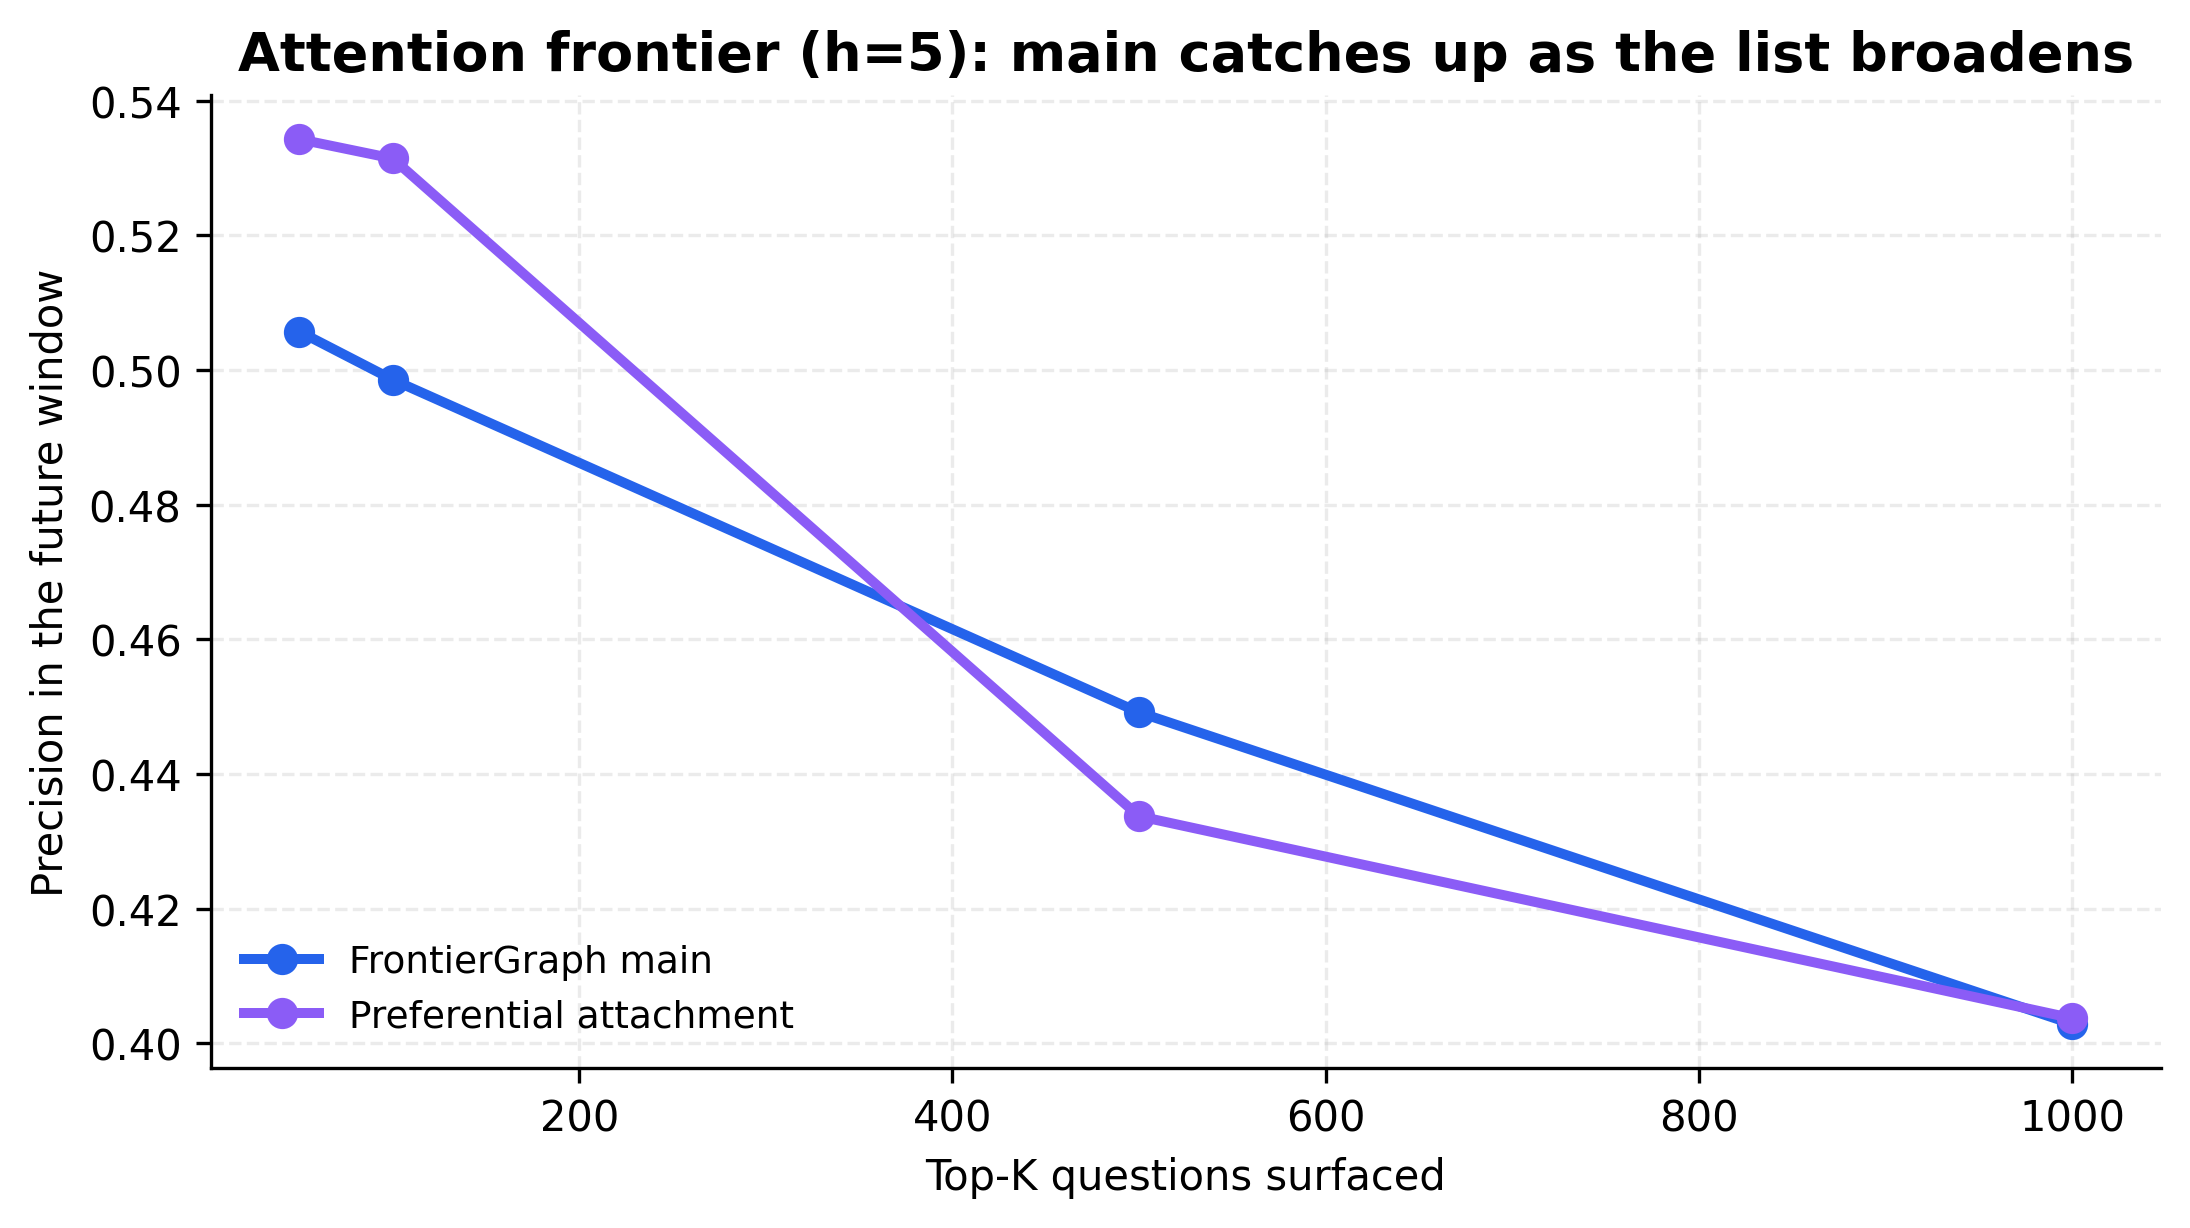
\includegraphics[width=\linewidth]{attention_allocation_frontier.png}

\column{0.38\linewidth}
\small
\begin{itemize}
  \item At very small \(K\), preferential attachment is stronger.
  \item As the surfaced list broadens, the transparent model catches up and can slightly exceed it.
  \item That is relevant for real topic-search workflows, where economists rarely consume just one suggestion.
\end{itemize}
\end{columns}
\end{frame}

\begin{frame}[label=app-impact]{A11. Impact-weighted evaluation}
\appendixnav{main-whyinteresting}
\vspace{0.35em}
\begin{columns}[T]
\column{0.56\linewidth}
\includegraphics[width=\linewidth]{../outputs/paper/08_impact_weighted/impact_weighted_recall_frontier_h5.png}

\column{0.40\linewidth}
\small
\begin{itemize}
  \item Weight future links by later impact, not only binary realization.
  \item The transparent model does not dominate here either, but the gap changes under weighted evaluation.
  \item This matters if the paper wants to move from ``does it appear?'' to ``does it matter when it appears?''
\end{itemize}
\end{columns}
\end{frame}

\begin{frame}[label=app-gap]{A12. Gap vs boundary decomposition}
\appendixnav{main-surfaces}
\vspace{0.35em}
\begin{columns}[T]
\column{0.56\linewidth}
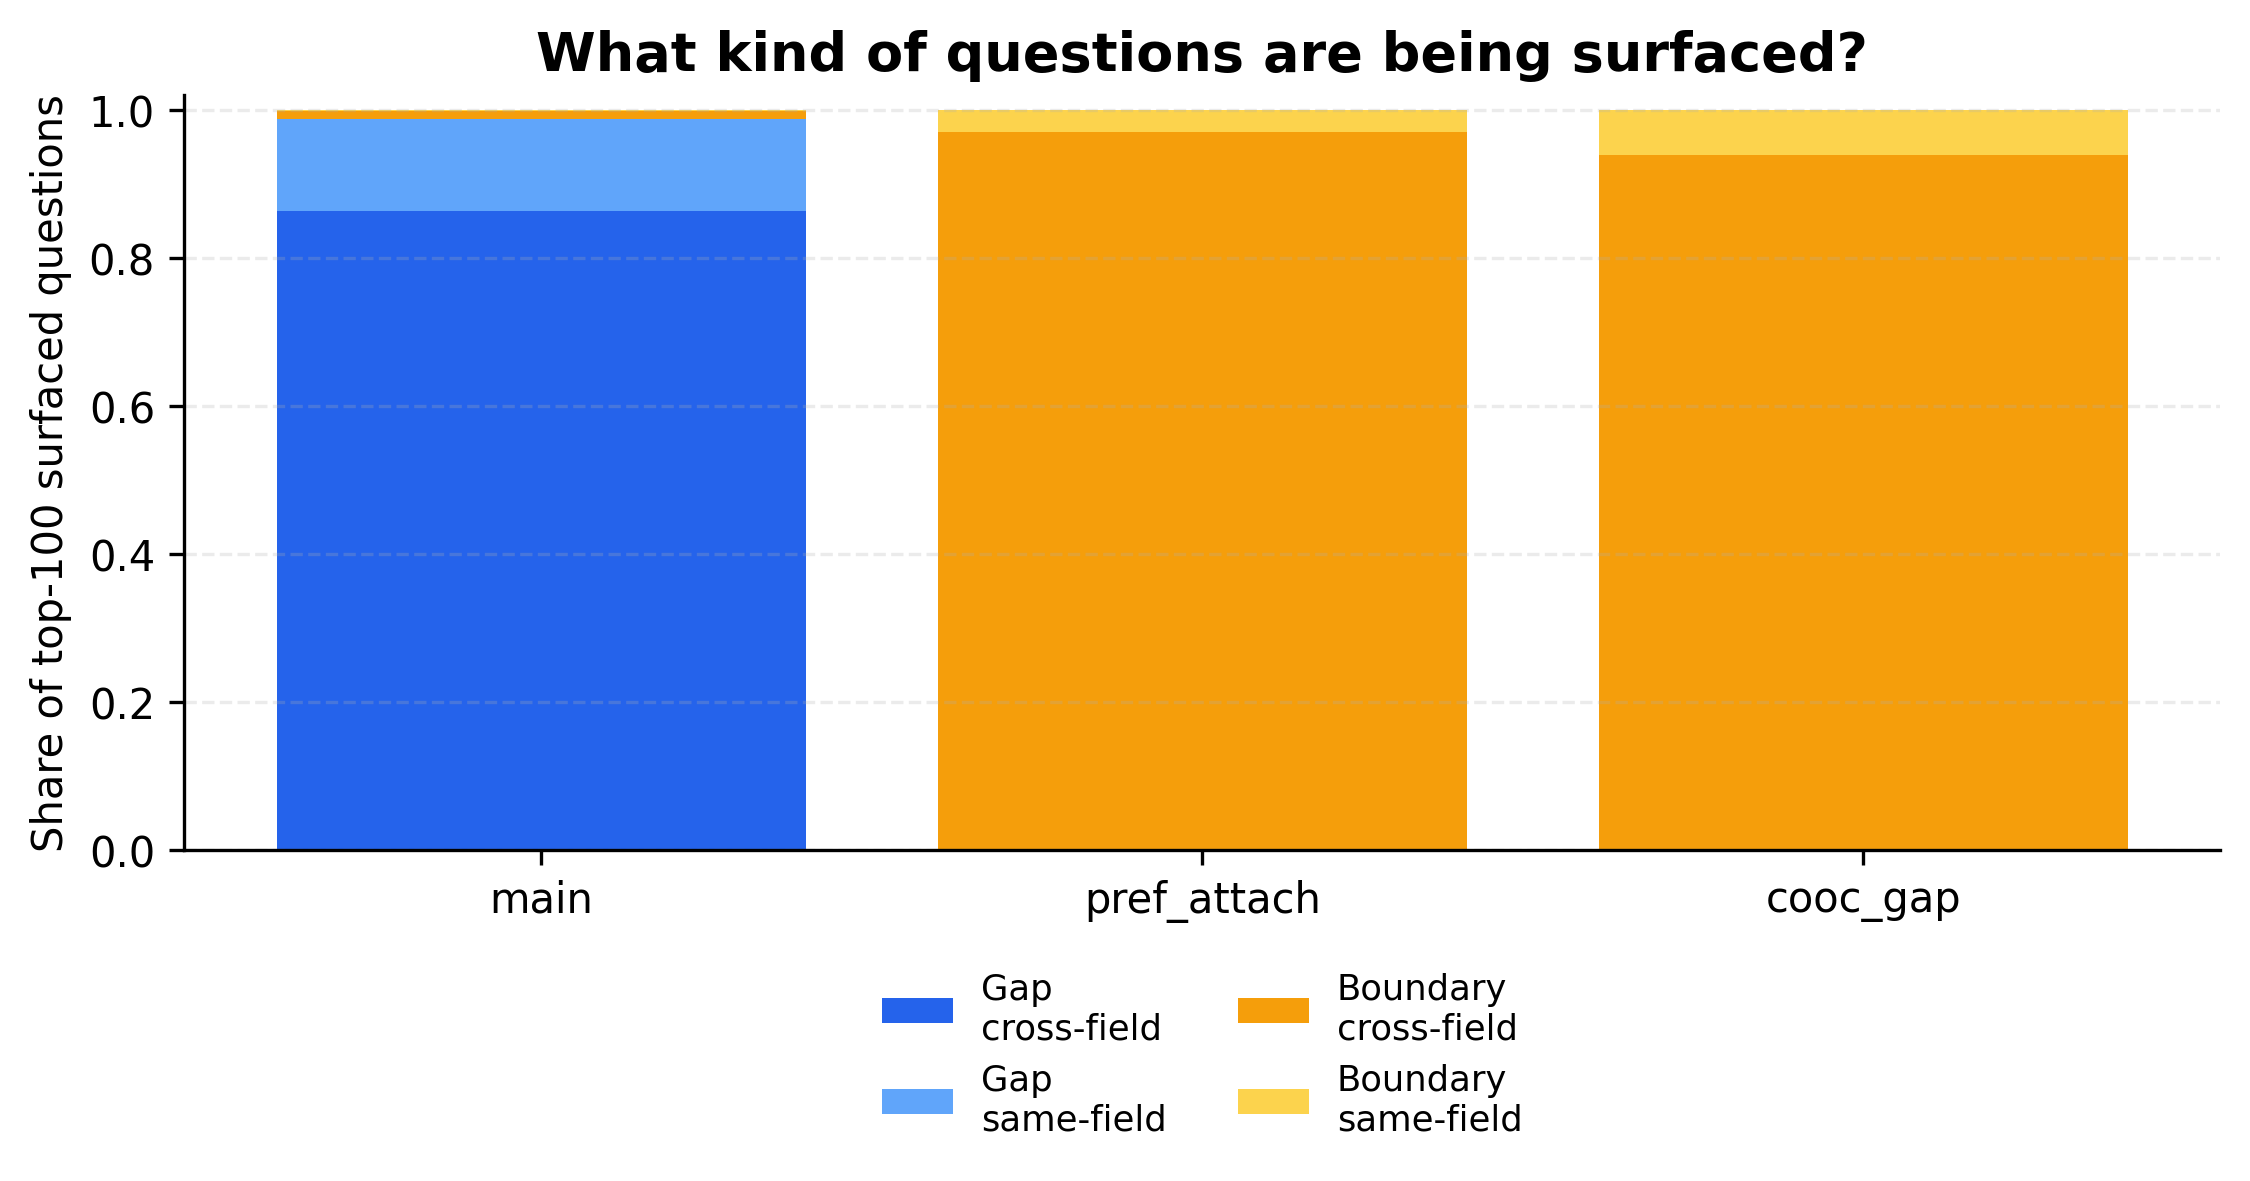
\includegraphics[width=\linewidth]{gap_boundary_mainline.png}

\column{0.40\linewidth}
\small
\begin{itemize}
  \item In the top-100, the transparent model concentrates on gap-type questions.
  \item Preferential attachment is overwhelmingly boundary-crossfield in this decomposition.
  \item This decomposition helps explain why the two systems behave differently, even before asking which one wins on realization.
\end{itemize}
\end{columns}
\end{frame}

\begin{frame}[label=app-heterogeneity]{A13. Field heterogeneity}
\appendixnav{main-surfaces}
\vspace{0.35em}
\begin{columns}[T]
\column{0.64\linewidth}
\includegraphics[width=\linewidth]{field_heterogeneity.png}

\column{0.32\linewidth}
\small
Realization rates differ sharply across fields.

\vspace{0.4em}
That is one reason a single overall score is not enough for substantive interpretation.
\end{columns}
\end{frame}

\begin{frame}[label=app-examples]{A14. More examples and case diagnostics}
\appendixnav{main-examples}
\small
\begin{itemize}
  \item \textbf{Public debt and CO\(_2\) emissions}: macro-fiscal stress spilling into climate outcomes.
  \item \textbf{Monetary policy and energy consumption}: sectoral energy demand as an overlooked transmission channel.
  \item \textbf{Urbanization and output growth}: a development question often treated as background rather than the outcome itself.
  \item \textbf{Investment and carbon emissions}: likely better treated as a question family than a single narrow pair.
\end{itemize}

\vspace{0.4em}
\small
These examples are best used as illustrative outputs of the current FrontierGraph layer, not as evidence that the historical backtest has already validated these exact questions.
\end{frame}

\begin{frame}[label=app-transfer]{A15. External transfer design}
\appendixnav{main-next}
\vspace{0.35em}
\begin{columns}[T]
\column{0.48\linewidth}
\textbf{Design directions}
\begin{itemize}
  \item OpenAlex economics-tagged works
  \item RePEc / IDEAS / NBER
  \item IMF / World Bank / OECD research corpora
  \item Patent-linked transfer tests
\end{itemize}

\column{0.48\linewidth}
\textbf{Why this matters}
\begin{itemize}
  \item Separate internal predictability from external generalization.
  \item Test whether the research-allocation story survives outside one corpus build.
  \item Pre-register horizons and evaluation discipline.
\end{itemize}
\end{columns}
\end{frame}

\begin{frame}[label=app-lockbox]{A16. Expert validation and prospective lockbox}
\appendixnav{main-next}
\vspace{0.35em}
\begin{columns}[T]
\column{0.48\linewidth}
\begin{block}{Expert validation}
\small
\begin{itemize}
  \item Blind experts to system arm
  \item Compare main vs pref vs random
  \item Rate novelty-adjusted priority
\end{itemize}
\end{block}

\column{0.48\linewidth}
\begin{block}{Prospective lockbox}
\small
\begin{itemize}
  \item Freeze predictions with a manifest hash
  \item Score future realization later
  \item Prevent moving-goalpost evaluation
\end{itemize}
\end{block}
\end{columns}

\vspace{0.35em}
\small
If this becomes a paper, these two pieces are the cleanest route from an interesting prototype to a stronger scientific claim.
\end{frame}

\end{document}
